\documentclass[12pt]{article}
%%---------------------------------------------------------------------
% packages
% geometry
\usepackage{geometry}
% font
\usepackage{fontspec}
\defaultfontfeatures{Mapping=tex-text}  %%如果没有它,会有一些 tex 特殊字符无法正常使用,比如连字符。
\usepackage{xunicode,xltxtra}
\usepackage[BoldFont,SlantFont,CJKnumber,CJKchecksingle]{xeCJK}  % \CJKnumber{12345}: 一万二千三百四十五
\usepackage{CJKfntef}  %%实现对汉字加点、下划线等。
\usepackage{pifont}  % \ding{}
% math
\usepackage{amsmath,amsfonts,amssymb}
% color
\usepackage{color}
\usepackage{xcolor}
\definecolor{EYE}{RGB}{199,237,204}
\definecolor{FLY}{RGB}{128,0,128}
\definecolor{ZHY}{RGB}{139,0,255}
% graphics
\usepackage[americaninductors,europeanresistors]{circuitikz}
\usepackage{tikz}
\usetikzlibrary{positioning,arrows,shadows,shapes,calc,mindmap,trees,backgrounds}  % placements=positioning
\usepackage{graphicx}  % \includegraphics[]{}
\usepackage{subfigure}  %%图形或表格并排排列
% table
\usepackage{colortbl,dcolumn}  %% 彩色表格
\usepackage{multirow}
\usepackage{multicol}
\usepackage{booktabs}
\usepackage{tcolorbox}
% code
\usepackage{fancyvrb}
\usepackage{listings}
\lstset{language=C++}%这条命令可以让LaTeX排版时将C++键字突出显示
\lstset{breaklines}%这条命令可以让LaTeX自动将长的代码行换行排版
\lstset{extendedchars=false}
% title
\usepackage{titlesec}
% head/foot
\usepackage{fancyhdr}
% ref
\usepackage{hyperref}
% pagecolor
\usepackage[pagecolor={EYE}]{pagecolor}
% tightly-packed lists
\usepackage{mdwlist}

\usepackage{styles/iplouccfg}
\usepackage{styles/zhfontcfg}
\usepackage{styles/iplouclistings}

%%---------------------------------------------------------------------
% settings
% geometry
\geometry{left=2cm,right=1cm,top=2cm,bottom=2cm}  %设置 上、左、下、右 页边距
\linespread{1.5} %行间距
% font
\setCJKmainfont{Adobe Kaiti Std}
%\setmainfont[BoldFont=Adobe Garamond Pro Bold]{Apple Garamond}  % 英文字体
%\setmainfont[BoldFont=Adobe Garamond Pro Bold,SmallCapsFont=Apple Garamond,SmallCapsFeatures={Scale=0.7}]{Apple Garamond}  %%苹果字体没有SmallCaps
\setCJKmonofont{Adobe Fangsong Std}
% graphics
\graphicspath{{figures/}}
\tikzset{
    % Define standard arrow tip
    >=stealth',
    % Define style for boxes
    punkt/.style={
           rectangle,
           rounded corners,
           draw=black, very thick,
           text width=6.5em,
           minimum height=2em,
           text centered},
    % Define arrow style
    pil/.style={
           ->,
           thick,
           shorten <=2pt,
           shorten >=2pt,},
    % Define style for FlyZhyBall
    FlyZhyBall/.style={
      circle,
      minimum size=6mm,
      inner sep=0.5pt,
      ball color=red!50!blue,
      text=white,},
    % Define style for FlyZhyRectangle
    FlyZhyRectangle/.style={
      rectangle,
      rounded corners,
      minimum size=6mm,
      ball color=red!50!blue,
      text=white,},
    % Define style for zhyfly
    zhyfly/.style={
      rectangle,
      rounded corners,
      minimum size=6mm,
      ball color=red!25!blue,
      text=white,},
    % Define style for new rectangle
    nrectangle/.style={
      rectangle,
      draw=#1!50,
      fill=#1!20,
      minimum size=5mm,
      inner sep=0.1pt,}
}
\ctikzset{
  bipoles/length=.8cm
}
% code
\lstnewenvironment{VHDLcode}[1][]{%
  \lstset{
    basicstyle=\footnotesize\ttfamily\color{black},%
    columns=flexible,%
    framexleftmargin=.7mm,frame=shadowbox,%
    rulesepcolor=\color{blue},%
%    frame=single,%
    backgroundcolor=\color{yellow!20},%
    xleftmargin=1.2\fboxsep,%
    xrightmargin=.7\fboxsep,%
    numbers=left,numberstyle=\tiny\color{blue},%
    numberblanklines=false,numbersep=7pt,%
    language=VHDL%
    }\lstset{#1}}{}
\lstnewenvironment{VHDLmiddle}[1][]{%
  \lstset{
    basicstyle=\scriptsize\ttfamily\color{black},%
    columns=flexible,%
    framexleftmargin=.7mm,frame=shadowbox,%
    rulesepcolor=\color{blue},%
%    frame=single,%
    backgroundcolor=\color{yellow!20},%
    xleftmargin=1.2\fboxsep,%
    xrightmargin=.7\fboxsep,%
    numbers=left,numberstyle=\tiny\color{blue},%
    numberblanklines=false,numbersep=7pt,%
    language=VHDL%
    }\lstset{#1}}{}
\lstnewenvironment{VHDLsmall}[1][]{%
  \lstset{
    basicstyle=\tiny\ttfamily\color{black},%
    columns=flexible,%
    framexleftmargin=.7mm,frame=shadowbox,%
    rulesepcolor=\color{blue},%
%    frame=single,%
    backgroundcolor=\color{yellow!20},%
    xleftmargin=1.2\fboxsep,%
    xrightmargin=.7\fboxsep,%
    numbers=left,numberstyle=\tiny\color{blue},%
    numberblanklines=false,numbersep=7pt,%
    language=VHDL%
    }\lstset{#1}}{}
% pdf
\hypersetup{pdfpagemode=FullScreen,%
            pdfauthor={Haiyong Zheng},%
            pdftitle={Title},%
            CJKbookmarks=true,%
            bookmarksnumbered=true,%
            bookmarksopen=false,%
            plainpages=false,%
            colorlinks=true,%
            citecolor=green,%
            filecolor=magenta,%
            linkcolor=cyan,%red(default)
            urlcolor=cyan}
% section
%http://tex.stackexchange.com/questions/34288/how-to-place-a-shaded-box-around-a-section-label-and-name
\newcommand\titlebar{%
\tikz[baseline,trim left=3.1cm,trim right=3cm] {
    \fill [cyan!25] (2.5cm,-1ex) rectangle (\textwidth+3.1cm,2.5ex);
    \node [
        fill=cyan!60!white,
        anchor= base east,
        rounded rectangle,
        minimum height=3.5ex] at (3cm,0) {
        \textbf{\thesection.}
    };
}%
}
\titleformat{\section}{\Large\bf\color{blue}}{\titlebar}{0.1cm}{}
% head/foot
\setlength{\headheight}{15pt}
\pagestyle{fancy}
\fancyhf{}
%\lhead{\color{black!50!green}2014年秋季学期}
\chead{\color{black!50!green}Zooplankton Identification}
%\rhead{\color{black!50!green}通信电子电路}
\lfoot{\color{blue!50!green}戴嘉伦\ 武斌\ 朱亚菲\ 王如晨}
\cfoot{\color{blue!50!green}\href{http://vision.ouc.edu.cn/~zhenghaiyong}{CVBIOUC}}
\rfoot{\color{blue!50!green}$\cdot$\ \thepage\ $\cdot$}
\renewcommand{\headrulewidth}{0.4pt}
\renewcommand{\footrulewidth}{0.4pt}


%%---------------------------------------------------------------------
\begin{document}
%%---------------------------------------------------------------------
%%---------------------------------------------------------------------
% \titlepage
\title{\vspace{-2em}浮游动物识别\vspace{-0.7em}}
\author{戴嘉伦\ 武斌\ 朱亚菲\ 王如晨}
\date{\vspace{-0.7em}2015年6月\vspace{-0.7em}}
%%---------------------------------------------------------------------
\maketitle\thispagestyle{fancy}
%%---------------------------------------------------------------------
\maketitle
\tableofcontents 

%\section{ZooScan系统}

由法国国家科学研究院Villefranche海洋实验室的Gorsky等人发明~\cite{gorsky2003qualitative}、Hydroptic公司生产的ZooScan浮游动物图像扫描分析系统是一种实验室成像系统(即针对的是已经采集并固定保存的浮游生物样品),主要用于对液体中的浮游动物样品进行计数、大小测量、种类鉴定以及生物量测定。ZooScan系统采用非破坏性技术对液体浮游动物样本进行分析,样品可重复使用。

ZooScan系统是由ZooScan、ZooProcess和Plankton Identifier(PkID)等共同组成的,ZooScan是硬件部分,主要进行浮游动物样品扫描,形成数字图像。ZooProcess和PkID是软件部分,分别以标准化的程序处理原始图像、对不同个体的形态参数进行自动测量和对图像中的浮游动物进行自动分类和计数。

\section{ZooScan扫描仪}

ZooScan扫描仪完成的任务:
\begin{itemize}
\item 扫描空白背景
\item 扫描样品,获得原始图片和元数据信息
\end{itemize}

\subsection{操作步骤}
\subsubsection{创建项目}
\begin{itemize}
\item 打开``Image J'',在软件界面中,选择项目选项表最后的 ``CREATE NEW PROJECT'',创建一个新的项目。如图~\ref{fig:create}。
    \begin{figure}[!ht]
    \centering
    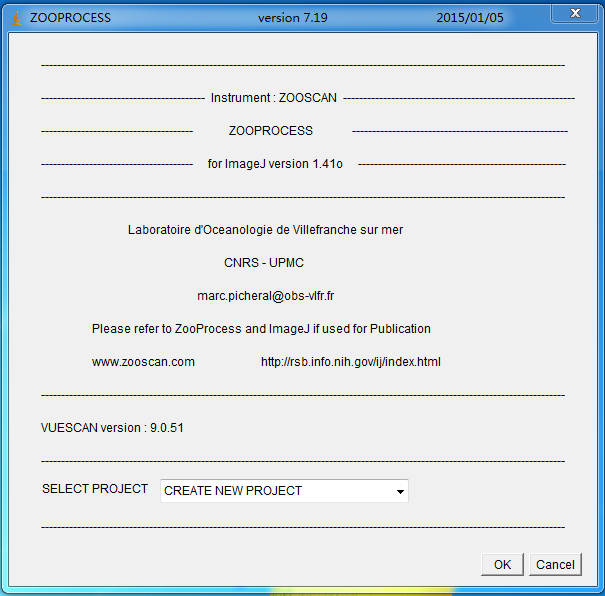
\includegraphics[width=3in]{create}
    \caption{创建项目}
    \label{fig:create}
    \end{figure}
\item 选择扫描选项。选择2400dpi分辨率和``Large''的扫描框(15$cm$ $\times$ 24$cm$)。如图~\ref{fig:frame}。
    \begin{figure}[!ht]
    \centering
    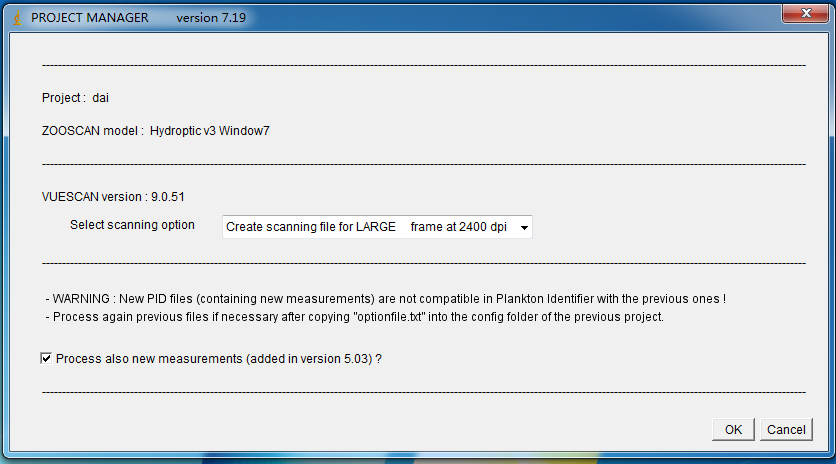
\includegraphics[width=3.5in]{frame}
    \caption{选择分辨率和扫描框大小}
    \label{fig:frame}
    \end{figure}
\item 输入样品的元数据(metadata)。在后面处理过程中,可以通过ZooProcess中的\textbf{``EDIT and MODIFY metadata''}工具来修改元数据。如图~\ref{fig:metadata}。
    \begin{figure}[!ht]
    \centering
    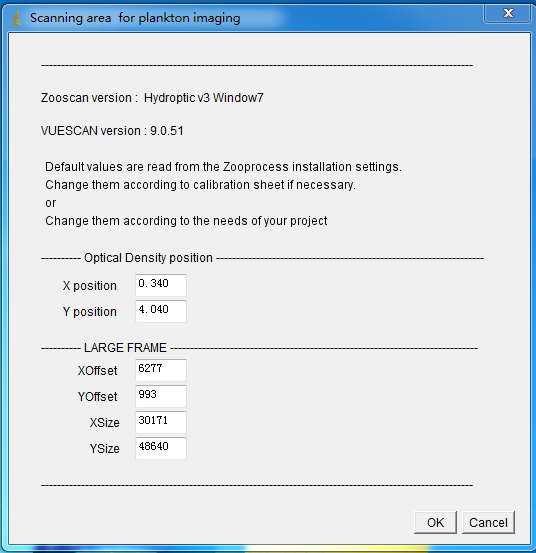
\includegraphics[width=3.0in]{metadata}
    \caption{输入扫描信息}
    \label{fig:metadata}
    \end{figure}
\end{itemize}


\subsubsection{扫描背景}
背景图像是一张空白图像,用于图像分析过程中。在与样品相同环境下 (自来水或是过滤海水),先扫描背景再扫描样品。最好是在每个扫描任务开始时,都扫描一次背景图像。
\begin{itemize}
\item 用清水清洁和冲洗ZooScan托盘和表面玻璃,时不时地检查并清除在玻璃和扫描框上的污点。
\item 倒一些清水(保持在室温)没过托盘,它可以防止扫描框刮擦托盘。
\item 放置扫描框(15$cm$ $\times$ 24$cm$),这取决于之前ZooProcess中的``创建项目''中的选项。
\item 在预扫描和实际扫描之间,等待30秒。
\end{itemize}

\subsubsection{准备样品}
\begin{itemize}
\item 存储几升清水,保持在室温,用来为ZooScan注水。
\item 用筛子(网格间隙为100$\mu m$ )过滤掉防腐剂和海水中物质。样品通过间隙为1$mm$和200$\mu m$的两种网格,将浮游生物分成不同体型的两部分。
%%\item 用木棒将粘连的浮游生物分离开,且避免浮游生物贴靠扫描框边缘。
\item 浮游生物被分为不同体型的两部分:一个为体型大的样品,另一个为体型小的样品。分别将分开后的样品,添加标签$d1$和$d2$,用于扫描后的数据处理过程中。如图~\ref{fig:volume}。
  \begin{figure}[!ht]
  \centering
   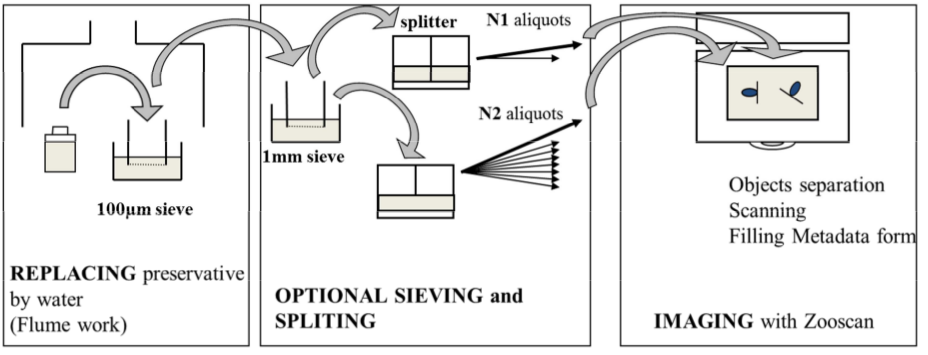
\includegraphics[width=3.6in]{volume}
    \caption{准备样品}
    \label{fig:volume}
   \end{figure}
\item 使上述两个分开后的样品中,保持只有1000 $ - $ 1500个浮游生物。
\end{itemize}

\subsubsection{扫描样品}
\begin{itemize}
\item 在扫描托盘中加入量水,放置扫描框(15$cm$ $\times$ 24$cm$),调整扫描框放置的位置(位置在扫描托盘中有标注)。
\item 倒入样品,加入清水,直到没过扫描框的台阶。
\item 将个体较大的浮游生物放在扫描框的中心,用木棒分离粘连浮游生物,避免浮游生物贴靠扫描框边缘。对于漂浮在水面的浮游生物,轻轻用木棒将浮游生物压入水中。如果存在无法没入水中的浮游动物,且数量不多,则将它们移出 ({\color{blue} 这一步是生成好的数据质量的关键步骤})。如图~\ref{fig:sticks}。
  \begin{figure}[!ht]
  \centering
   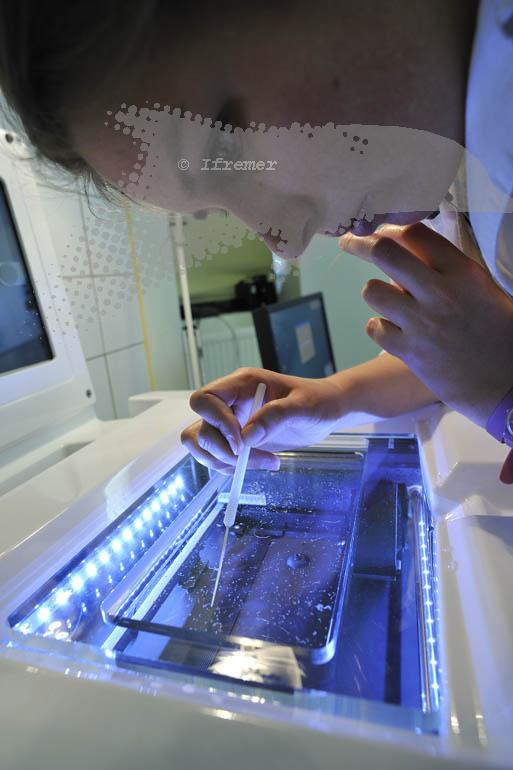
\includegraphics[width=2.0in]{sticks}
    \caption{用木棒分离粘连浮游生物}
    \label{fig:sticks}
   \end{figure}
\item 检查托盘是否有气泡,顶盖玻璃的表面是否冷凝。
\item 加载ZooProcess,选择项目,点击扫描样品,选择两部分样品中的一个样品($d1$和$d2$),写入相关元数据。
\end{itemize}

\subsubsection{回收样品}
\begin{itemize}
\item 清洁托盘,避免下次实验污染了样品。
\item 移走并冲洗透明的扫描框,回收所有的标本。
\item 清洁干燥扫描托盘。
\end{itemize}


\subsection{注意事项}
\begin{itemize}
\item 清水可以是自来水或过滤海水,保持在室温是为了避免在ZooScan的托盘中产生气泡或者顶盖玻璃上出现冷凝。因为自来水管中的自来水和房间的温度存在一定温差。
\item ZooScan提供1200dpi和2400dpi两种分辨率扫描。分辨率限制在2400dpi,是由于ZooScan设计的光路需要空气入水和由水进入玻璃两次穿过界面,使成像分辨率收到限制。
\item ZooScan的扫描框有两个尺寸:11$cm$ $\times$ 24$cm$ 和 15$cm$ $\times$ 24$cm$。推荐使用15$cm$ $\times$ 24$cm$的扫描框,具体使用哪个扫描框由ZooProcess中的选项决定。
\item 扫描空白背景不仅可以去除灯光产生的异质性的斑点等,而且可以检验系统的稳定性。
%%\item 防止大个且数量较少的浮游生物被低估
\item 在准备样品阶段,通常情况下,将样品分为两个或以上的小样品进行扫描。
\item 在准备样品阶段,如何将浮游生物样品分成不同的小样品,取决于原样品中浮游生物的种类多少与体型大小。
\item 扫描的浮游生物必须保持不动的状态,使用固定剂或将其麻醉。
\item 扫描框上有5mm的小台阶,注入的水必须漫过这台阶的高度,避免在扫描后的图像边缘出现弯液面现象。如图~\ref{fig:step}。
  \begin{figure}[!ht]
  \centering
   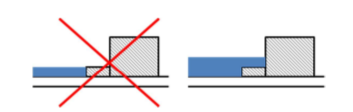
\includegraphics[width=2.8in]{step.png}
    \caption{框的台阶高度}
    \label{fig:step}
   \end{figure}
\item 在较大的框内(15$cm$ $\times$ 24$cm$),最多可以容纳1000 $ - $ 1500个浮游生物。
\item 在ZooProcess中也可以对扫描图像中的粘连浮游生物进行分离,但是最好是在样品扫描之前用木棒进行分离。如图~\ref{fig:separate}。
  \begin{figure}[!ht]
  \centering
   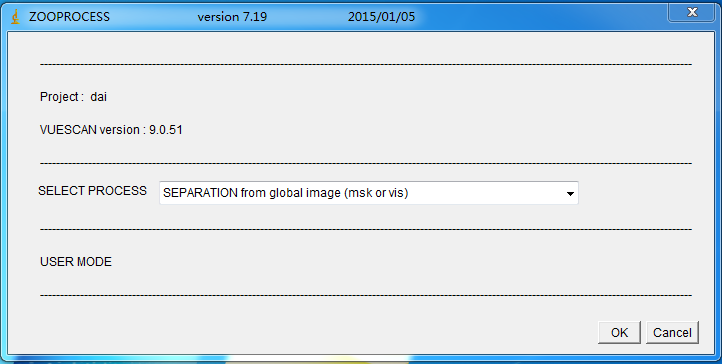
\includegraphics[width=3.5in]{separate}
    \caption{ZooProcess的浮游生物分离}
    \label{fig:separate}
   \end{figure}
\end{itemize}

\section{ZooProcess}
ZooProcess介绍详见\url{http://wbtxd2004.github.io/zooscan/2015/06/13/Zooprocess-Study.html}。

%\subsection{Free software ZooProcess Using ImageJ}
%
%ImageJ\footnote{\url{http://rsb.info.nih.gov/ij/index.html}}是一个基于java的公共的图像处理软件,它是由National Institutes of Health开发的。除了基本的图像操作,比如缩放,旋转,扭曲,平滑处理外,ImageJ还能进行图片的区域和像素统计,间距,角度计算,能创建柱状图和剖面图,进行傅里叶变换。
%
%ZooProcess中用到的一些变量如下:
%
%\begin{description}
%\item[Angle] Angle between the primary axis and a line parallel to the $x$-axis of the image 

%\item[X] X position of the center of gravity of the object 
%\item[XM] X position of the center of gravity of the object's grey level
%\item[XMg5] X position of the center of gravity of the object, using a gamma value of 51

%\item[Y] Y position of the center of gravity of the object 
%\item[YM] Y position of the center of gravity of the object's grey level
%\item[YMg5] Y position of the center of gravity of the object, using a gamma value of 51


%\item[Slope] 标准化灰度累计直方图的斜率
%\item[Histcum1] grey level value at 25\% of the normalized cumulative histogram of grey levels
%\item[Histcum2] grey level value at 50\% of the normalized cumulative histogram of grey levels
%\item[Histcum3] grey level value at 75\% of the normalized cumulative histogram of grey levels

%\item[IntDen] Integrated density. The sum of the grey values of the pixels in the object (i.e. $1⁄4$ Area*Mean) \item[Median] Median grey value within the object

%\item[\%area] Percentage of object's surface area that is comprised of holes, defined as the background grey level
%\item[Area\_exc] Surface area of the object excluding holes, in square pixels ($1⁄4$Area*(12(\%area/100)) 


%\end{description}
%
%5、扫描“背景”图片
%
%背景图片是一幅空白图片,在后续图像处理过程中会用到。背景扫描应该安排在样本扫描之前,并且在同样的条件或环境下进行。建议在每次的扫描环节开始之前都要先进行背景图片的扫描。
%
%基本步骤如下:
%
%\begin{itemize}
%\item 打开ZooSCAN,如果有必要的话用清水冲洗扫描托盘和盖玻片。
%\item 时不时检查盖玻片,看是否有痕迹,以便擦去。
%\item 
%\end{itemize}

\section{Plankton Identifier(PkID)}

\subsection{主窗口}

打开PkID应用程序,显示的界面上共有5个按钮:“Learning”、“Evaluation”、“Prediction”、“Validation”和“Compilation”(图~\ref{fig: Main window})。这5个部分可以相互独立地运行,但是会有运行的先后顺序。比如“Evaluation”和“Prediction”会用到“Learning”生成的文件,“Validation”用到“Prediction”生成的文件,“Compilation”用到“Validation”所生成的文件。因此,当你第一次使用PkID时你应该首先运行“Learning”。

\begin{figure}[!ht]
\centering
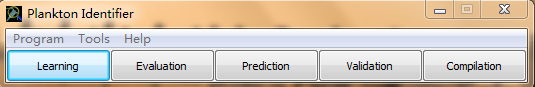
\includegraphics[width=0.8\textwidth]{mainWindow.png}
\caption{主窗口}
\label{fig: Main window}
\end{figure} 

其他菜单:

\textit{\textbf{Program > Settings}} 定义Tanagra.exe所在的路径以及存放缩略图、PID文件和结果的默认文件夹路径。

Tanagra Path:如果你安装了两个以上的Tanagra版本,你可以选择想要使用的版本。点击\textbf{Browse},浏览硬盘文件夹,找到Tanagra.exe,点击\textbf{OK}。

\textit{注:如果你的Tanagra没有安装在 $\backslash$Program Files$\backslash$Tanagra 路径下,或者你就根本没有安装Tanagra,这时当你运行PkID时就会自动弹出这个窗口(图~\ref{fig: Settings window})。}

\begin{figure}[!ht]
\centering
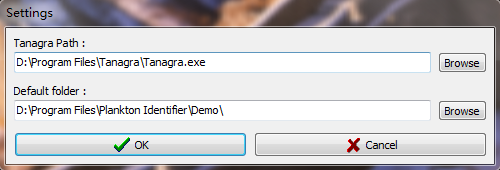
\includegraphics[width=0.7\textwidth]{settingsWindow.png}
\caption{设置窗口}
\label{fig: Settings window}
\end{figure} 

Default folder:默认文件夹是你第一次使用PkID执行一些步骤产生的文件所存放的地方。

\textit{\textbf{Program > Exit}} 关闭PkID。

\subsection{Learning}

这一步会生成一个学习文件以用作后续的自动识别。它对应于经专家鉴定的具有代表性的一些物体的子样本并且可以作为将来分析的参考。

1、文件夹选择窗口

当点击\textbf{Learning}按钮时,会出现如图~\ref{fig: SelectLearningSetFolderWindow}所示的文件夹选择窗口。 

\begin{figure}[!ht]
\centering
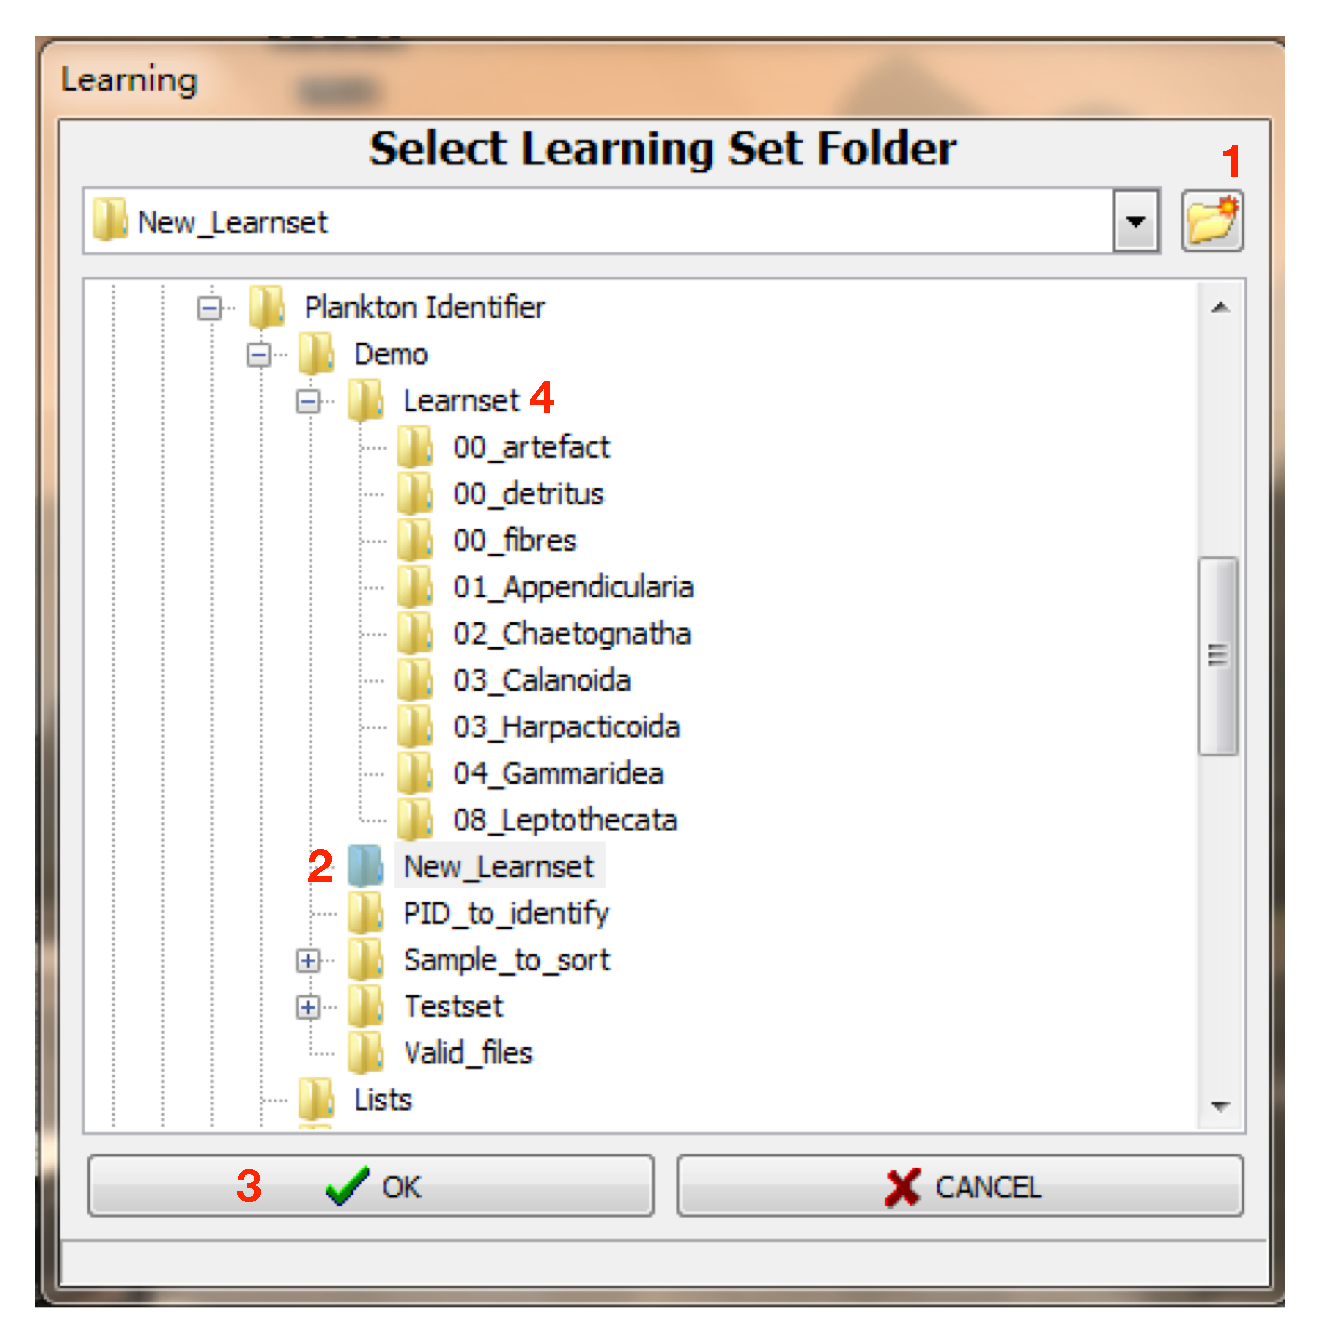
\includegraphics[width=0.6\textwidth]{SelectLearningSetFolderWindow.eps}
\caption{训练集文件夹选择窗口}
\label{fig: SelectLearningSetFolderWindow}
\end{figure} 

选择一个空的文件夹以用来创建新的训练数据集,你也可以通过点击右上角的按钮(图~\ref{fig: SelectLearningSetFolderWindow}: {\color{red}\textbf{1}})来创建一个新的文件夹然后给它命名(图~\ref{fig: SelectLearningSetFolderWindow}: {\color{red}\textbf{2}}),最后点击\textbf{OK}按钮(图~\ref{fig: SelectLearningSetFolderWindow}: {\color{red}\textbf{3}})。

你也可以选择一个已有的训练数据集(其中包含已分类好的子文件夹以及包含物体元数据的一些PID格式的文件,每个子文件夹代表一个种类,其中存放属于该类的jpg格式的缩略图),如图~\ref{fig: SelectLearningSetFolderWindow}: {\color{red}\textbf{4}}。

{\color{blue}\textit{注:如果此处选择的文件夹结构不符,或者包含了无效的数据,那么将会无法打开,并且在窗口的最下方会出现一行红色的警告信息以说明原因。}}

2、学习窗口

当选择了一个可以用来对缩略图进行分类的有效文件夹之后,点击\textbf{OK},会出现一个新的窗口(图~\ref{fig: LearningWindow})。其中左边部分(“Sample Set”)是要通过浏览硬盘文件夹来选择未被分类的样本。右边部分(“Learning Ser”)是要将左边未被分类的样本拖到右边以完成分类(创建子文件夹)。

\begin{figure}[!ht]
\centering
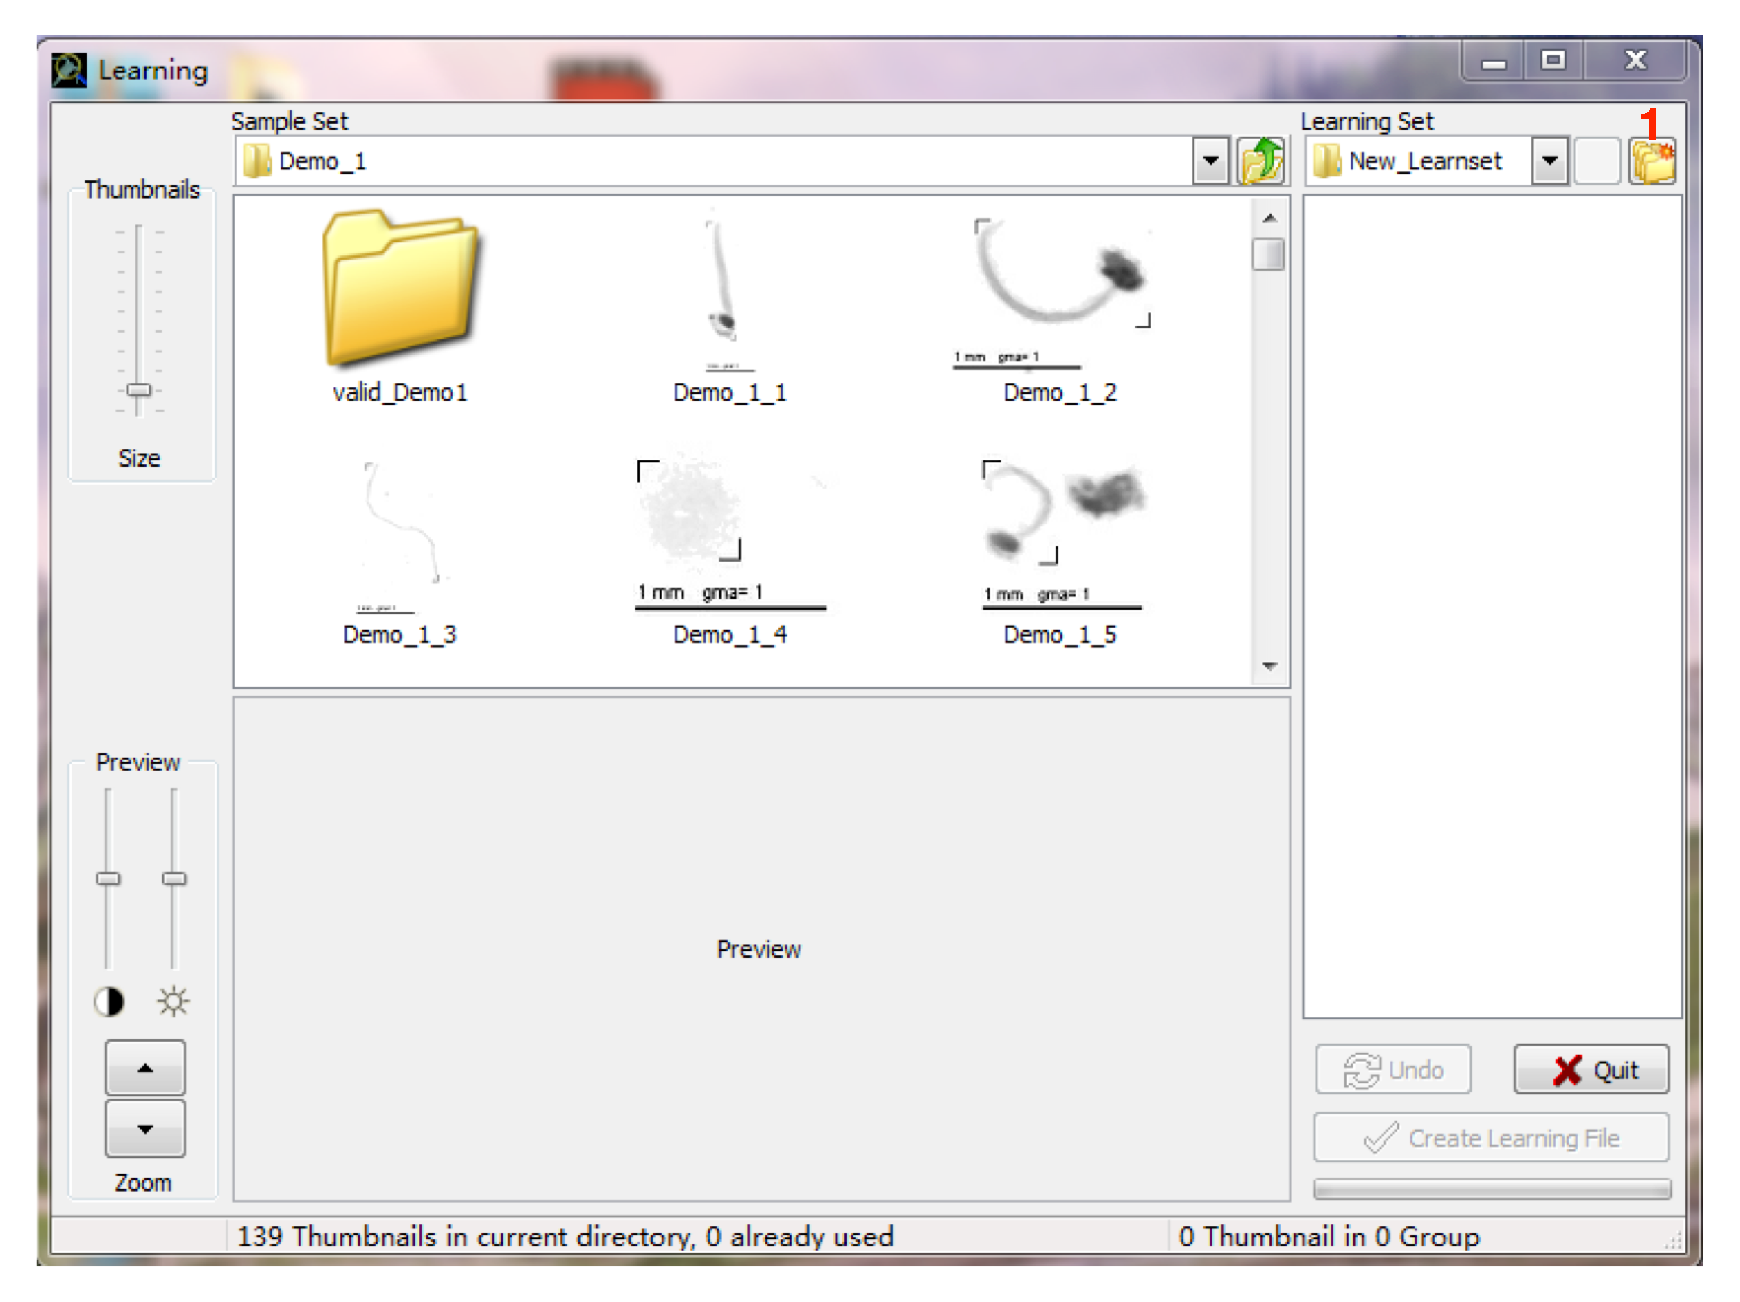
\includegraphics[width=0.6\textwidth]{LearningWindow.eps}
\caption{Learning窗口}
\label{fig: LearningWindow}
\end{figure} 

\textit{Sample Set}

在窗口左边栏“Sample Set”处,浏览硬盘文件夹以打开一个包含未分类的缩略图和相应PID文件的文件夹。只有有有效名字(<Sample Name>\_<Item Number>.jpg)的缩略图才会在左边栏中显示出来。如果名字是有效的但是PID文件中并没有包含该幅图像的一些数据,这时就会这个缩略图上方会出现一个问号并且当把鼠标放在问号上时会有相应的原因解释,这幅图也是无法使用的。

\textit{注:如果此处选择的文件夹结构不符,或者包含了无效的数据,那么将会无法打开,并且在窗口的最下方会出现一行红色的警告信息以说明原因。}

\textit{类别(子文件夹)创建}

在窗口右边栏“Learning Set”处,为了把缩略图归到对应的类别,需要在步骤1所选择的文件夹中创建一些子文件夹,每个文件夹代表一类。点击右上角的按钮(图~\ref{fig: LearningWindow}: {\color{red}\textbf{1}})创建新的文件夹,这时会出现一个新的窗口,可以给新创建的文件夹从给定的种类名字中选择一个(图~\ref{fig: CreateGroupsWindow})。如果给定的这些名字中没有合适的,你还可以选择另一个“Predefined Lists”或者先选择“New”作为名字,之后再在“Learning Set”这一栏中重新编辑命名。

\begin{figure}[!ht]
\centering
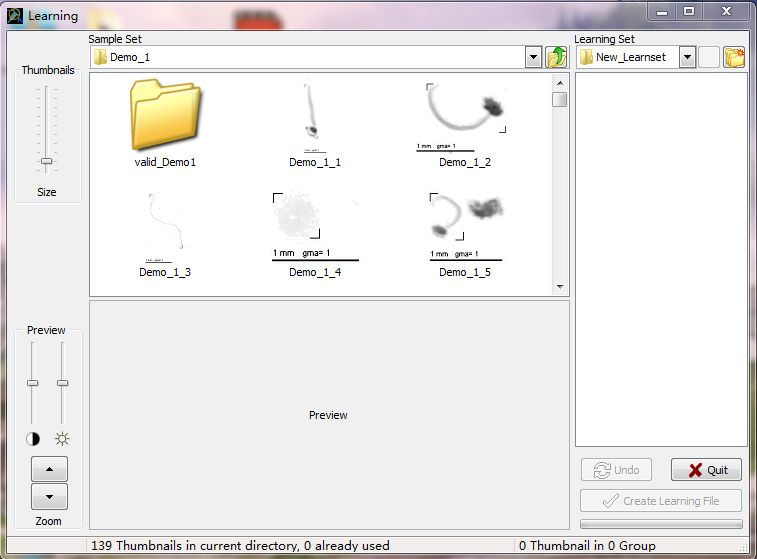
\includegraphics[width=0.6\textwidth]{LearningWindow.png}
\caption{创建训练集中分类类别的窗口}
\label{fig: CreateGroupsWindow}
\end{figure} 

{\color{blue}\textit{注1:所创建的子文件夹名字不能重复。已经用过的名字在“Create Group Folders”窗口中将不再显示。}}

{\color{blue}\textit{注2:可以通过\textbf{Tools>Import Name List}菜单来自定义你自己的种类名字清单。}}

\textit{对缩略图进行归类}

选中一个缩略图,下方会显示它的预览,如图~\ref{fig: ThumbnailsSorting}: {\color{red}\textbf{1}}。你可以通过左侧的\textbf{zoom}按钮(图~\ref{fig: ThumbnailsSorting}: {\color{red}\textbf{2}})将预览结果放大,还可以通过调节左侧对比度和亮度的状态条来显示更多细节。

\begin{figure}[!ht]
\centering
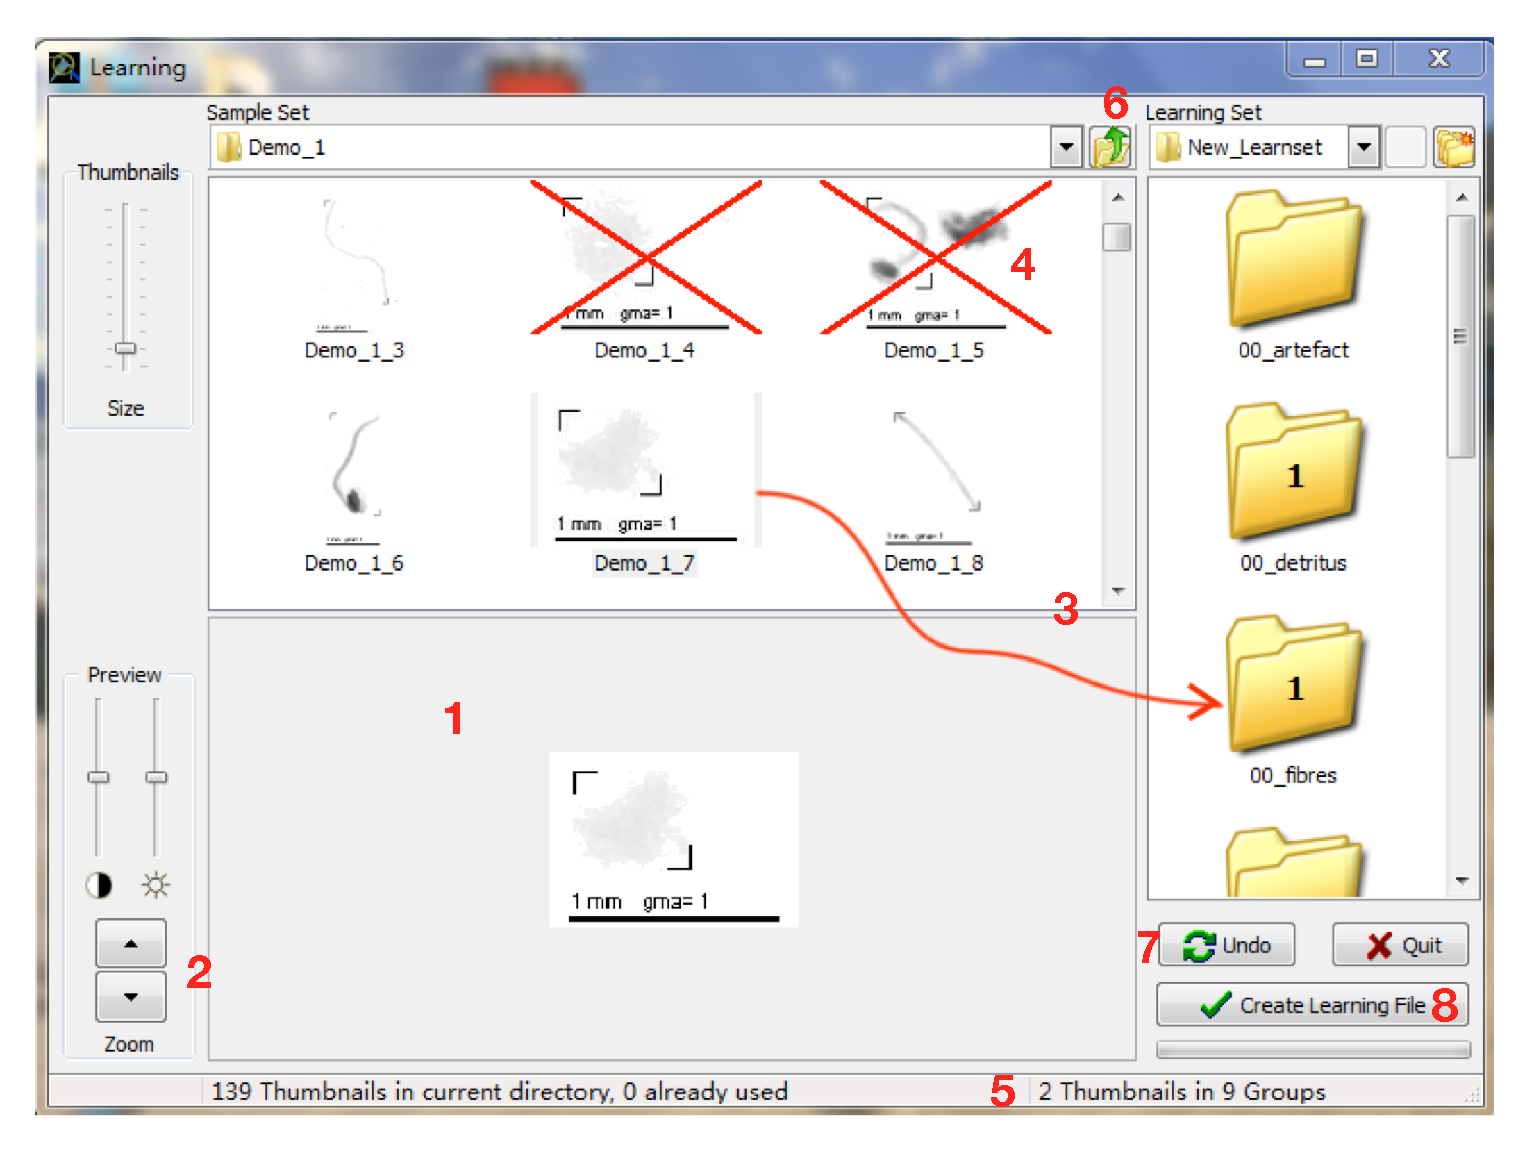
\includegraphics[width=0.7\textwidth]{ThumbnailsSorting.eps}
\caption{对样本文件中的缩略图进行分类}
\label{fig: ThumbnailsSorting}
\end{figure} 

把缩略图拖到相应的子文件夹中(图~\ref{fig: ThumbnailsSorting}: {\color{red}\textbf{3}}),这时缩略图会被复制到那个子文件夹中,而不是被剪切过去了。对应的PID文件也被复制到了右边文件夹中,但在这个窗口中是看不见的,以免视觉上的混淆。一旦一个缩略图已经用在了所创建的数据集中,上面就会出现一个红色的叉(图~\ref{fig: ThumbnailsSorting}: {\color{red}\textbf{4}}),表示它不能再被使用了。

一次选中多个缩略图也是可以的,可以通过按住Ctrl键来完成。在选中多个缩略图的时候,如果你想看每一个缩略图的预览效果,可以从右下角往左上角选择。

每一个子文件夹中缩略图的数目会显示在这个子文件夹上,并且随着你的操作而更新。已经被归类了的缩略图数目以及还没有完成归类的缩略图数目都被显示在了窗口的最下方(图~\ref{fig: ThumbnailsSorting}: {\color{red}\textbf{5}})。

你可以对多个样本集中的缩略图进行归类以创建自己的训练数据集。点击上面的一个按钮(图~\ref{fig: ThumbnailsSorting}: {\color{red}\textbf{6}})转到你想要操作的文件夹路径下。

\textit{Cancel action}

当你在训练数据集的创建过程中执行了一些误操作之后,可以有以下两个办法取消:(1)用\textbf{Undo}按钮(图~\ref{fig: ThumbnailsSorting}: {\color{red}\textbf{7}})(2)打开右侧的子文件夹,选中缩略图然后用DEL键删除。其中\textbf{Undo}键可以用来取消删除操作或子文件夹删除操作,DEL键可以用来删除一个所有缩略图都被清除了的空子文件夹。

\textit{创建学习文件}

一旦你觉得你创建的每一个类别中已经归类了足够多的样本,你就可以点击“Create Learning File”按钮(图~\ref{fig: ThumbnailsSorting}: {\color{red}\textbf{8}})了,点击之后会出现一个保存对话框,上面显示了所要保存的目标文件夹路径以及学习文件的名字,默认的名字为Learn\_<number>格式。点击“Save”按钮,所有的学习工作就完成了。这时又会出来一个会话框询问你是否要继续分类,如果你选择“No”,这个学习窗口就会被关闭回到主窗口。

\subsection{Evaluation}

这一步是要帮助你评估一下基于上一步中创建的训练数据集所建立的预测模型对训练数据集中的物体的识别率有多高。最后会生成一个包含识别结果的文本文件以及一个包含了数据分析信息的html报告。点击主窗口中的Evaluation按钮,会出现如下的界面(图~\ref{fig: EvaluationWindow})。

\begin{figure}[!ht]
\centering
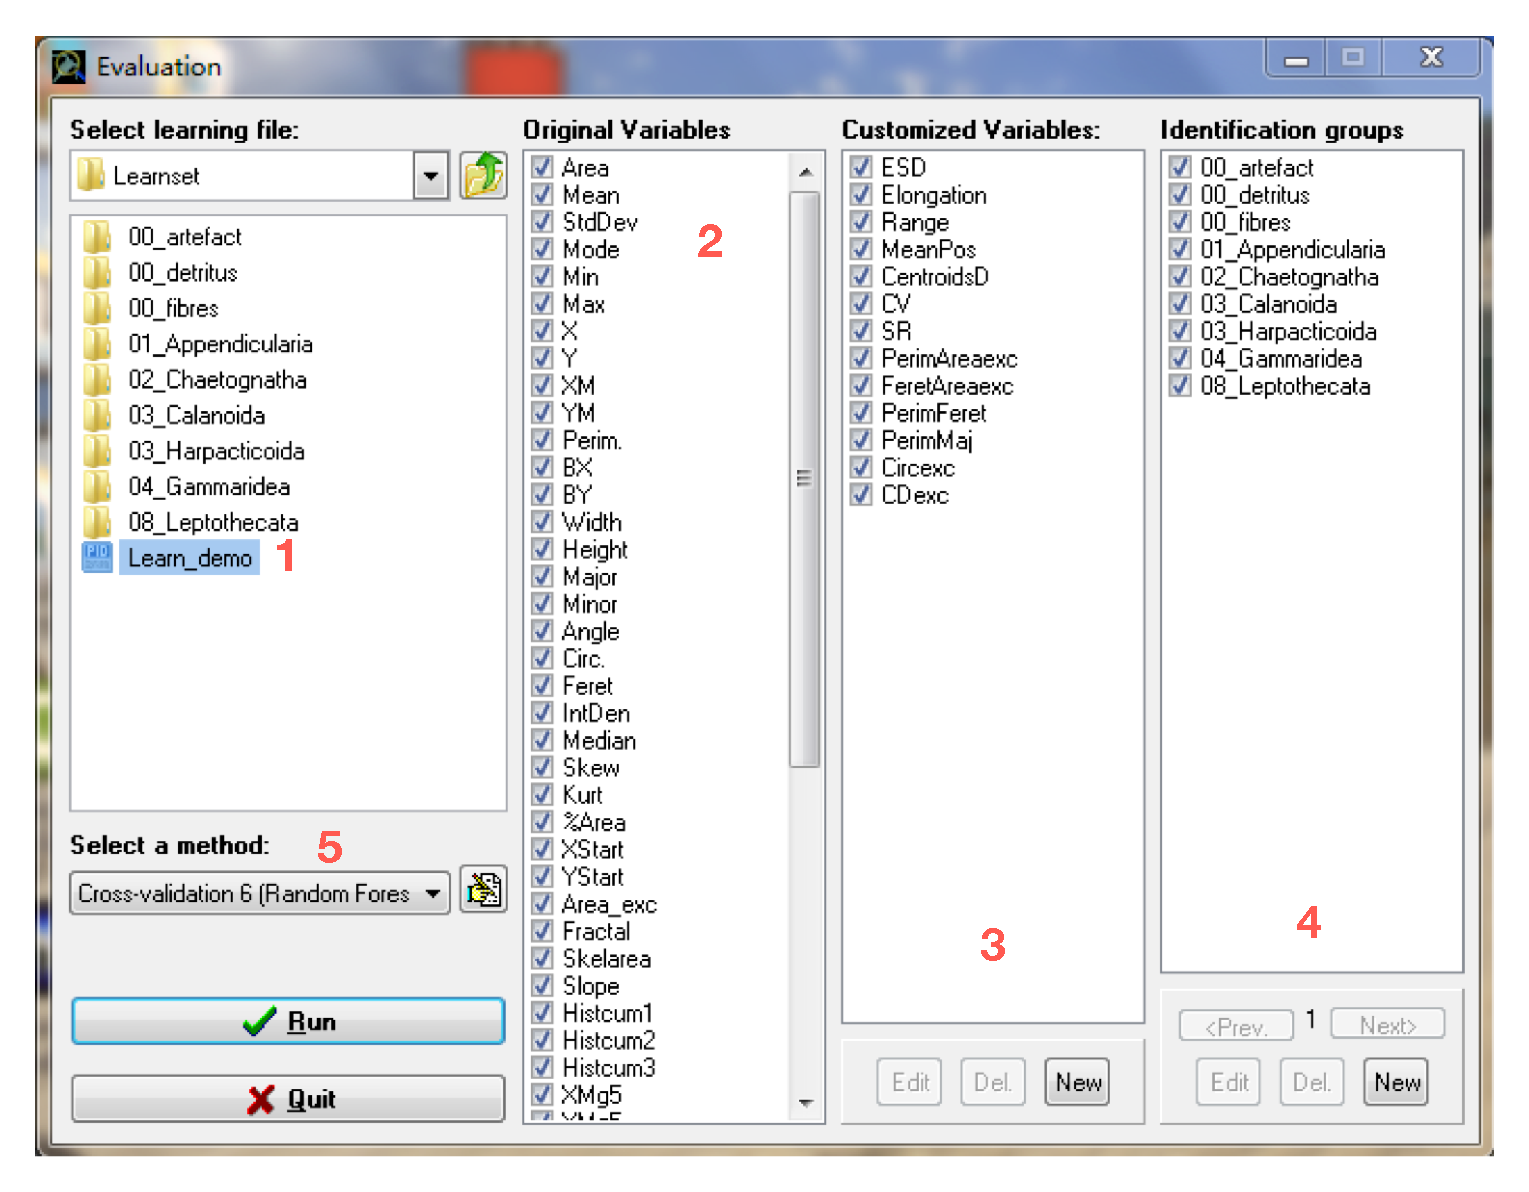
\includegraphics[width=0.7\textwidth]{EvaluationWindow.eps}
\caption{Evaluation窗口}
\label{fig: EvaluationWindow}
\end{figure} 

1、选取学习文件(图~\ref{fig: EvaluationWindow}: {\color{red}\textbf{1}})

浏览硬盘文件夹,选择你想要用来进行数据分析的学习文件。

{\color{blue}\textit{注1:选择学习文件后才能激活其它部分。}}

{\color{blue}\textit{注2:双击PID文件,将会自动在PID viewer(如果已安装)或者文本编辑器(例如Windows下的Notepad)中打开,从而可以校正文件内容。}}

2、初始变量(图~\ref{fig: EvaluationWindow}: {\color{red}\textbf{2}})

这里展示的是所选择的学习文件中的一些变量,你可以任意选取一些变量以用作分析,没有被选取的初始变量在计算时会被忽略,但不会从结果文件中移除。

{\color{blue}\textit{注:对于那些用ZooProcess软件生成的PID文件,在计算时要被忽略的初始变量可以在附件中找到。}}

3、自定义变量(图~\ref{fig: EvaluationWindow}: {\color{red}\textbf{3}})

这一步是要根据已有的初始变量创建自定义变量。在你安装PkID之后会有13个自定义变量可供你选择是否要用它。没有被选取的初始变量在计算时会被忽略,并且不会在结果文件中显示。如果定义的某个变量不能从已经选取的初始变量计算,那么它会自动变成不可选取状态,并且显示成灰色。

要编辑一个已经存在的自定义变量,选中它,点击\textbf{Edit}以打开一个新窗口(~\ref{fig: CustomizedVariableWindow})。

\begin{figure}[!ht]
\centering
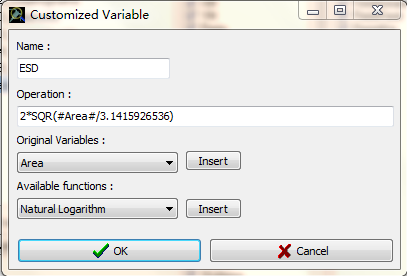
\includegraphics[width=0.7\textwidth]{CustomizedVariableWindow.png}
\caption{自定义变量窗口}
\label{fig: CustomizedVariableWindow}
\end{figure}

选中已存在的自定义变量,点击\textbf{Del}可以将其删除。

要新建一个自定义变量,点击\textbf{New},出现如图~\ref{fig: CustomizedVariableWindow}的变量自定义窗口。
\begin{enumerate}
\item 对新建的变量命名(命名必须与已有变量不同)
\item 在“Operation”下面一栏中输入计算公式
\item 按“OK”键
\end{enumerate}
{\color{blue}\textit{注:在编写公式时,一些基本的运算符(例如$+$, $-$, $\backslash$, $*$, $\^$)、括号、数字都是跟平常在键盘上敲的一样。要插入一个初始变量的话,可以在“Original Variables”下面一栏选中它,然后点击“Insert”。在公式中用到初始变量时,需要在这个初始变量前后加上“\#”号。在“Available functions”一栏中,可以选择一个函数进行插入。建议可以先看看已有的一些自定义变量是如何定义的,然后再编辑自己需要的公式。}}

4、Identification Groups(图~\ref{fig: EvaluationWindow}: {\color{red}\textbf{4}})

这里显示了在选取的学习文件中所定义的分类种类。默认的种类是不能被删除或编辑的,但是你可以通过将已有的类别合并来创建新的类别。

点击\textbf{New}可以创建新的类别,打开如图~\ref{fig: GroupsEditionWindow}所示的类别编辑窗口。

\begin{figure}[!ht]
\centering
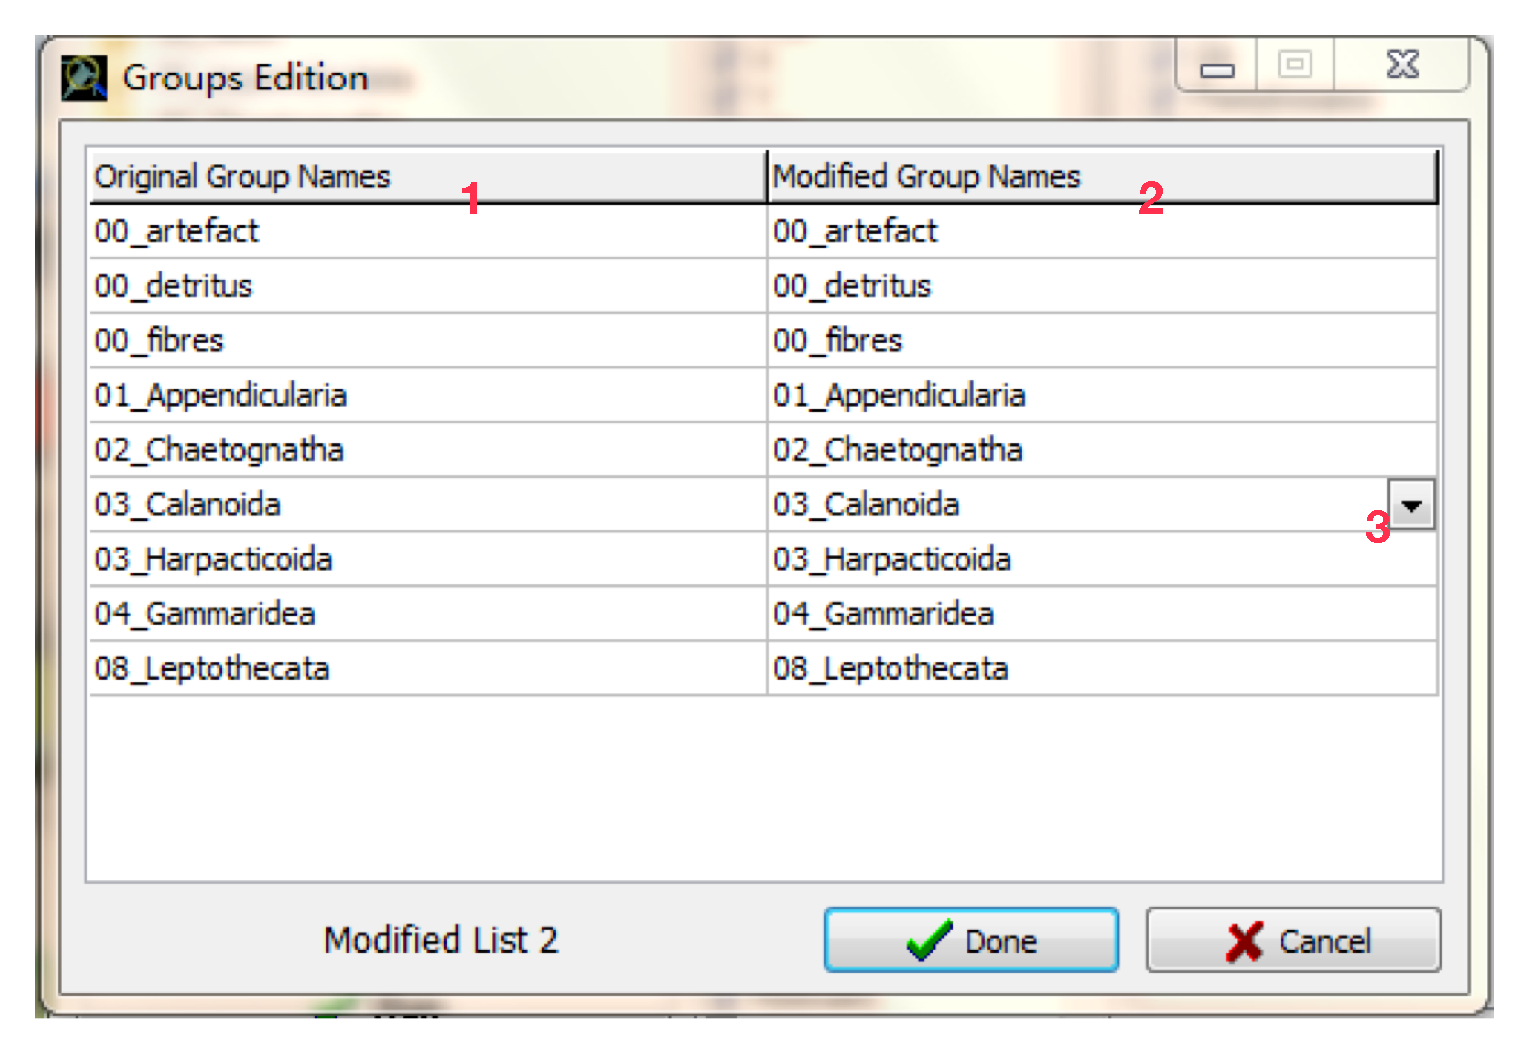
\includegraphics[width=0.7\textwidth]{GroupsEditionWindow.eps}
\caption{分类类别编辑窗口}
\label{fig: GroupsEditionWindow}
\end{figure}

修改初始类别名字(图~\ref{fig: GroupsEditionWindow}: {\color{red}\textbf{1}}):
\begin{enumerate}
\item 在“Modified Group Names”一栏下方选择一个需要修改的名字(图~\ref{fig: GroupsEditionWindow}: {\color{red}\textbf{2}})
\item 给这个类别重新编辑命名,或者点击如图(图~\ref{fig: GroupsEditionWindow}: {\color{red}\textbf{3}})所示按钮,在名字列表中选择一个
\item 完成对类别的重新命名后,点击\textbf{Done}
\end{enumerate}
{\color{blue}\textit{注:你可以创建很多的分类种类的列表,后续数据分析中用到的只会是当前这个列表(在Evaluation窗口点击\textbf{Run}时所看见的那个列表)。你可以用\textbf{Prev.}和\textbf{Next>}按钮来选择你想要的进行分析那个列表。在生成的结果文件中,初始名字会显示在“Ident1”这一列中,新的名字显示在“Ident2”这一列中。}}

5、选择一种方法(图~\ref{fig: EvaluationWindow}: {\color{red}\textbf{5}})

这里是要选择一种评价方法,用来检测用有监督学习方法和所选择的学习文件学习的模型的识别能力。PkID中一共提供了两种评价方法。

{\color{red}k-fold cross-validation method}:用重采样技术来评价学习算法在学习文件上的识别准确率。初始的训练数据集被随机分为$k$个相同大小的子集。每一次循环过程中,将$k-1$个子集放在一起形成训练集,并且构造出预测模型,剩下的那1个子集被当成测试集来评价模型预测能力。一共循环$k$次。这样下来,每个子集都会有1次机会作为测试集,$k-1$次机会作为训练集。将$k$次预测结果取平均,可以得到这个模型的最终预测能力。交叉验证过程会重复$n$次,$n$次交叉验证的平均错误率在一个混淆矩阵中被计算得到。

PkID一共实现了8种交叉验证方法,每一个都采用了不同的学习算法。

所有的交叉验证方法中所用的参数都是$k = 2, n = 5$。要想改变这两个值:

\begin{figure}[!ht]
\centering
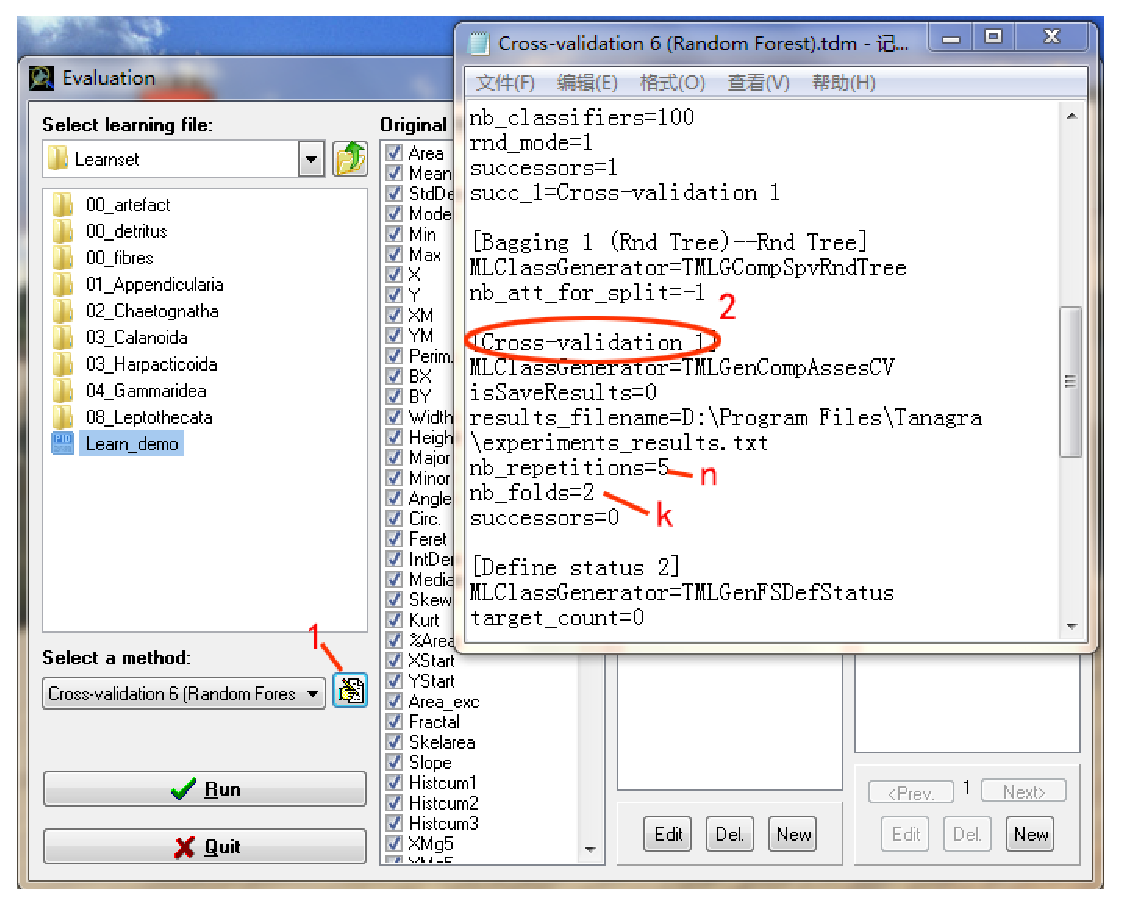
\includegraphics[width=0.7\textwidth]{ModificationofCrossValidationParameterisation.eps}
\caption{分类类别编辑窗口}
\label{fig: ModificationofCrossValidationParameterisation}
\end{figure}

\begin{enumerate}
\item 点击编辑按钮(图~\ref{fig: ModificationofCrossValidationParameterisation}: {\color{red}\textbf{1}}),打开相应的tdm文件
\item 在交叉验证部分修改$k$和$n$值图~\ref{fig: ModificationofCrossValidationParameterisation}: {\color{red}\textbf{2}}
\item 在关闭tdm文件前保存修改
\end{enumerate}

{\color{red}Test method}:在一个预先定义好的、独立的测试文件上对模型的准确率进行评价。在使用这个测试方法之前,需要创建一个特殊的文件,可以通过主窗口菜单中的\textbf{Concatenate Learning Files}来创建。相比于用两个不同的文件来作为训练集和测试集,我们更倾向于用一个文件来把它们联系起来,并且通过状态来表示所要扮演的角色,状态有“学习”和“测试”两种。

PkID提供了两种测试方法。Test 1可以通过在预先定义的测试文件上比较8个算法的准确率来选择最好的学习方法。Test 2只用到随机森林算法。

{\color{blue}\textit{注:通常来讲,训练集越大,所构造的分类模型越好,测试集越大,预测准确率越高。}}

{\color{red}Export to text file (no analysis)}:生成一个文本文件,包含了所选的学习文件中所有初始变量和自定义变量,而不包含预测结果。这个文件还可以输入到任意的数据挖掘软件站进行分析。

6、开始分析

当所有文件、变量、类别都选择好之后,点击\textbf{Run}按钮,将会出现一个保存页面,选择要保存的文件夹、文件名,点击\textbf{Save}。

分析完成后(可能需要几分钟,这取决于样本大小和所选方法),结果和html报告被保存在了所选择的文件夹中,并且html报告会自动在网页中打开。这时会有一个会话框询问你是否要退出Evaluation窗口,如果你选择“Yes”,Evaluation窗口就会被关闭并返回主窗口。

与初始PID文件相比,评价文件包含了以下新的列:
\begin{enumerate}
\item 对应于自定义变量的列
\item 包含了学习文件中分类类别的一列(Ident)
\item 包含了修改后的类别名字的一列(Ident2)
\item 用来表示状态的一列(Learning或Test)
\end{enumerate}

\subsection{Prediction}

这一步是要根据选择的学习文件中的种类对样本进行自动识别。结束后也会生成一个包含了自动识别结果的文本文件和一个包含了数据分析信息html报告。点击主窗口中的\textbf{Prediction}按钮,会打开一个新的窗口(图~\ref{fig: PredictionWindow}):

\begin{figure}[!ht]
\centering
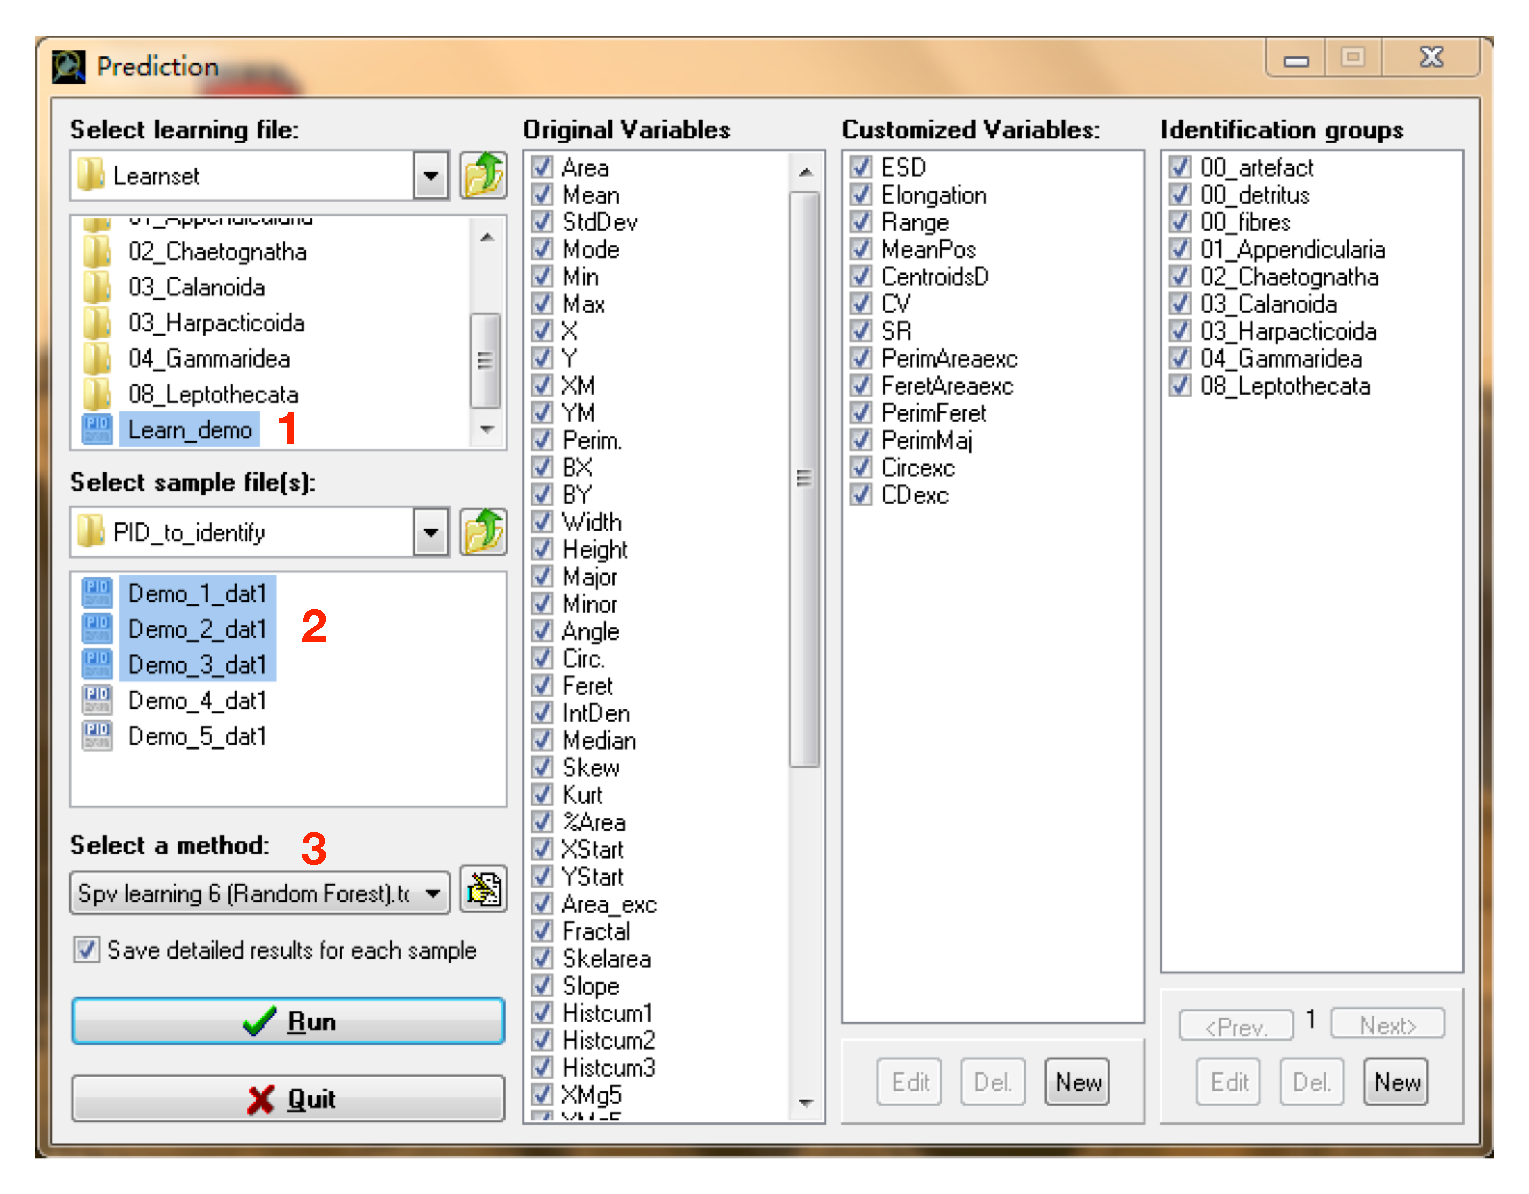
\includegraphics[width=0.7\textwidth]{PredictionWindow.eps}
\caption{Prediction窗口}
\label{fig: PredictionWindow}
\end{figure}

1、选择学习文件(图~\ref{fig: PredictionWindow}: {\color{red}\textbf{1}})

2、选择样本文件(图~\ref{fig: PredictionWindow}: {\color{red}\textbf{2}})

3、选择学习算法(图~\ref{fig: PredictionWindow}: {\color{red}\textbf{3}})

从PkID提供的8个学习算法中选择一个。
\begin{itemize}
\item Spv learning 1 (5-NN)
\item Spv learning 2 (C-SVC linear)
\item Spv learning 3 (C-SVC RBF)
\item Spv learning 4 (BVM)
\item Spv learning 5 (C4.5)
\item Spv learning 6 (Random Forest)
\item Spv learning 7 (PLS)
\item Spv learning 8 (Multilayer Perceptron)
\end{itemize}

4、开始分析

当所有文件、变量和分类类别都选好之后,点击\textbf{Run}按钮,会出现一个保存会话框。

\subsection{Validation}

这一步是将上一步生成的预测文件可视化,并且人为地对识别结果进行校正。这里可以有两个选择(图~\ref{fig: ValidationWindow}):1)用Prediction那一步生成的Pred\_.txt文件来将预测结果可视化,真正实现缩略图的自动分类,你还可以对自动识别的结果进行进一步检查和校正。2)打开一个已有的校正集来继续一个校正或进行二次校正。

\begin{figure}[!ht]
\centering
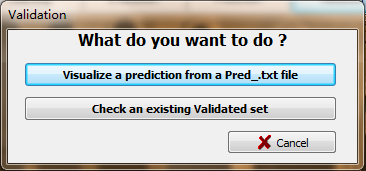
\includegraphics[width=0.7\textwidth]{ValidationWindow.png}
\caption{Validation窗口:What do you want to do?}
\label{fig: ValidationWindow}
\end{figure}

{\color{red}Visualize a prediction from a Pred\_.txt file}

\begin{figure}[!ht]
\centering
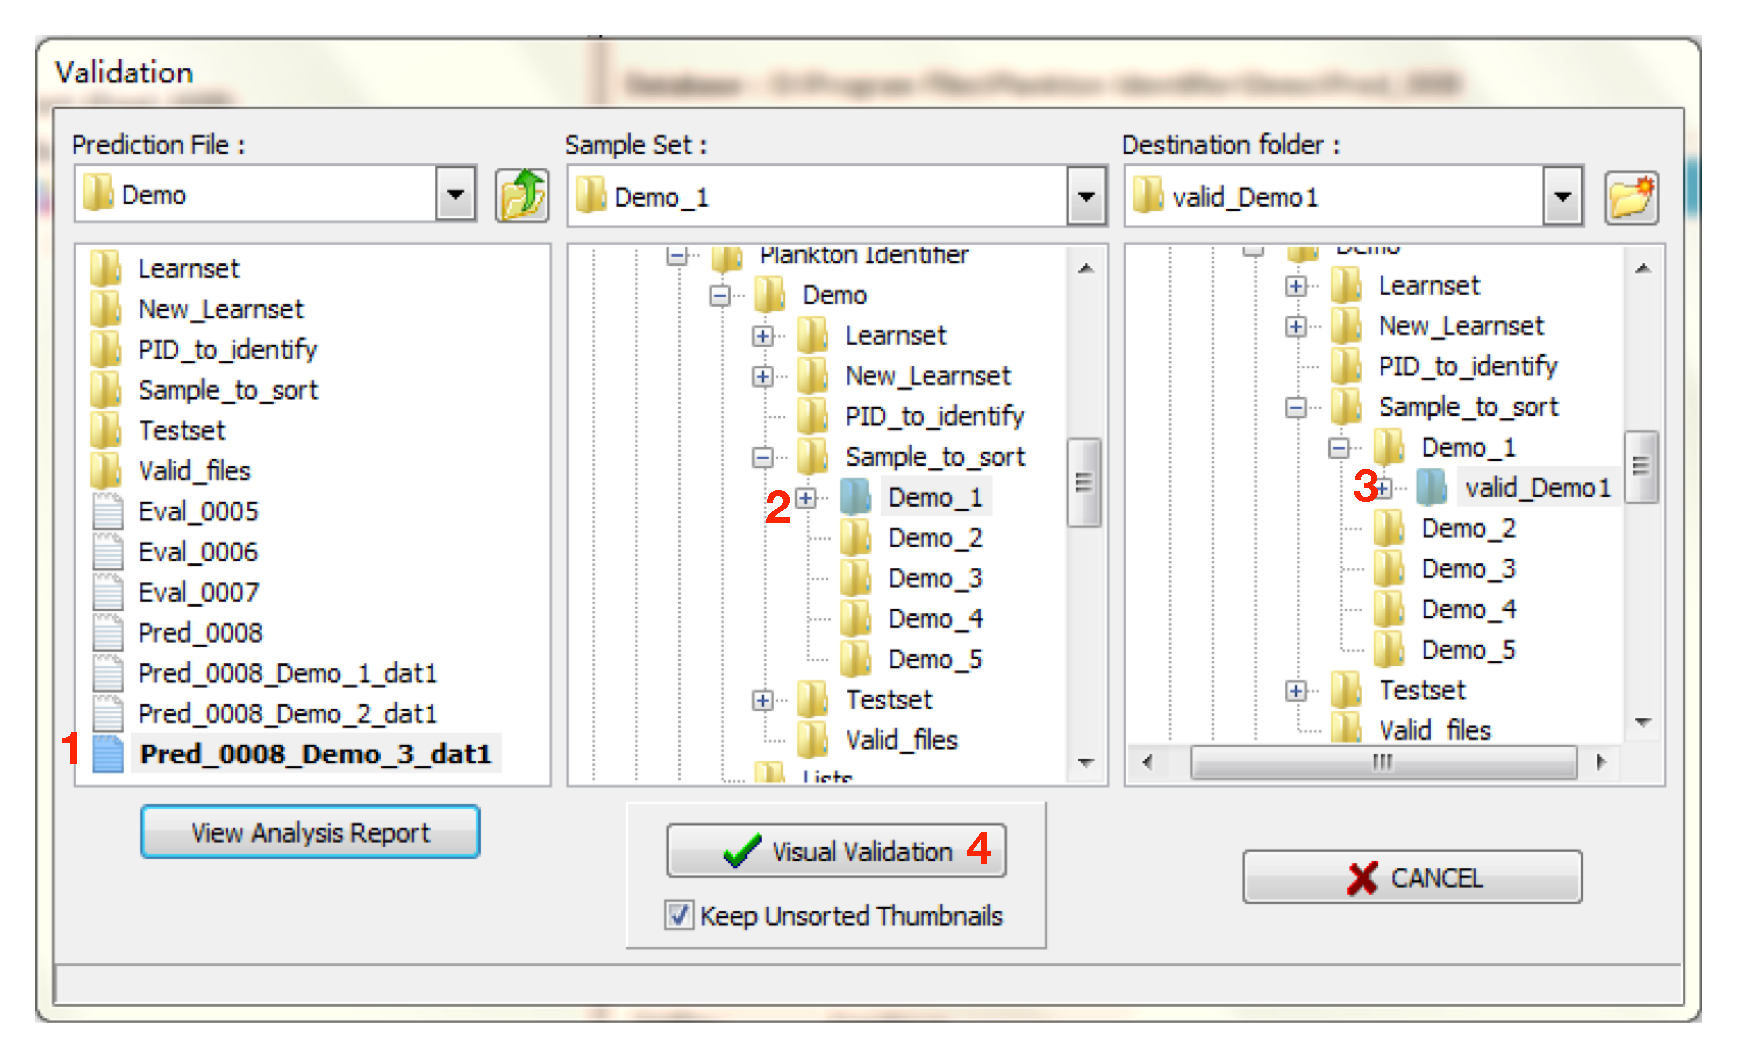
\includegraphics[width=0.7\textwidth]{SelectionWindowforValidation1.eps}
\caption{校正选择窗口1}
\label{fig: SelectionWindowforValidation1}
\end{figure}

\begin{enumerate}
\item 选择一个要用来校正的Pred\_.txt文件(图~\ref{fig: SelectionWindowforValidation1}: {\color{red}\textbf{1}})
\item 选择一个包含未分类缩略图的文件夹作为“Sample Set”(图~\ref{fig: SelectionWindowforValidation1}: {\color{red}\textbf{2}})
\item 选择用来存放分类好了的缩略图的目标文件夹(图~\ref{fig: SelectionWindowforValidation1}: {\color{red}\textbf{3}})
\item 点击“Visual Validation”(图~\ref{fig: SelectionWindowforValidation1}: {\color{red}\textbf{4}})
\end{enumerate}

{\color{blue}\textit{注:在分类过程中,缩略图是被复制而不是剪切到了目标文件夹中。如果你不想保留未分类的缩略图,可以在图~\ref{}处取消勾选\textbf{Keep Unsorted Thumbnails}。}}

{\color{red}Check an existing Validated set}

\begin{figure}[!ht]
\centering
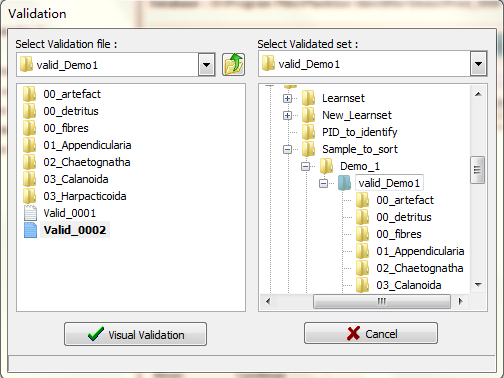
\includegraphics[width=0.7\textwidth]{SelectionWindowforValidation2.eps}
\caption{校正选择窗口2}
\label{fig: SelectionWindowforValidation2}
\end{figure}

\begin{enumerate}
\item 选择你想要检查的Valid\_.txt文件(图~\ref{fig: SelectionWindowforValidation2}: {\color{red}\textbf{1}})
\item 选择一个包含已分类好的校正后的缩略图的文件夹(图~\ref{fig: SelectionWindowforValidation2}: {\color{red}\textbf{2}})
\item 点击“Visual Validation”按钮(图~\ref{fig: SelectionWindowforValidation2}: {\color{red}\textbf{3}})
\end{enumerate}

{\color{red}Visual Validation}

前面的两个选择最终都会打开如图~\ref{fig: ValidationWindow2}所示的校正窗口:

\begin{figure}[!ht]
\centering
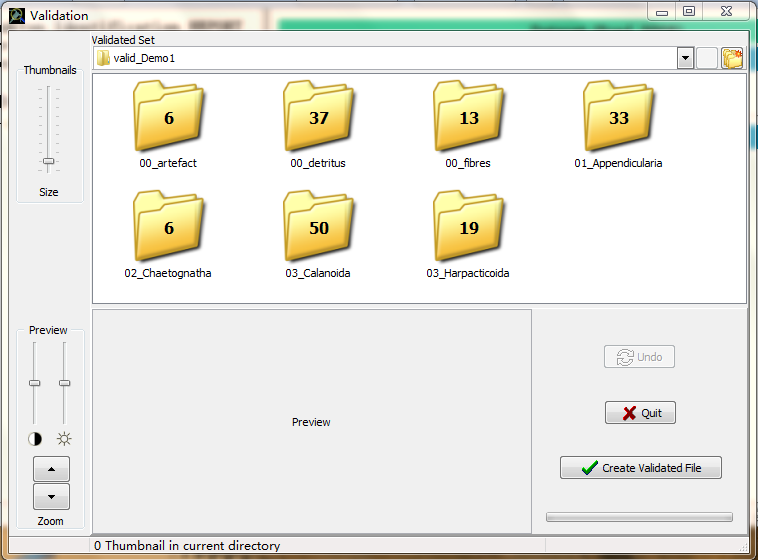
\includegraphics[width=0.7\textwidth]{ValidationWindow2.png}
\caption{校正窗口}
\label{fig: ValidationWindow2}
\end{figure}

利用预测模型已经将每幅缩略图放到了其对应的类别文件夹中,你可以打开每个文件夹查看是否被正确分类了。

{\color{red}Thumbnails moving}

\subsection{Compilation}

这一步是用来将上一步的生成的多个校正文件连起来,并且计算每个类别中的物体数目。在主窗口中点击\textbf{Compilation},会出现如下窗口(图~\ref{fig: CompilationWindow1}):

\begin{figure}[!ht]
\centering
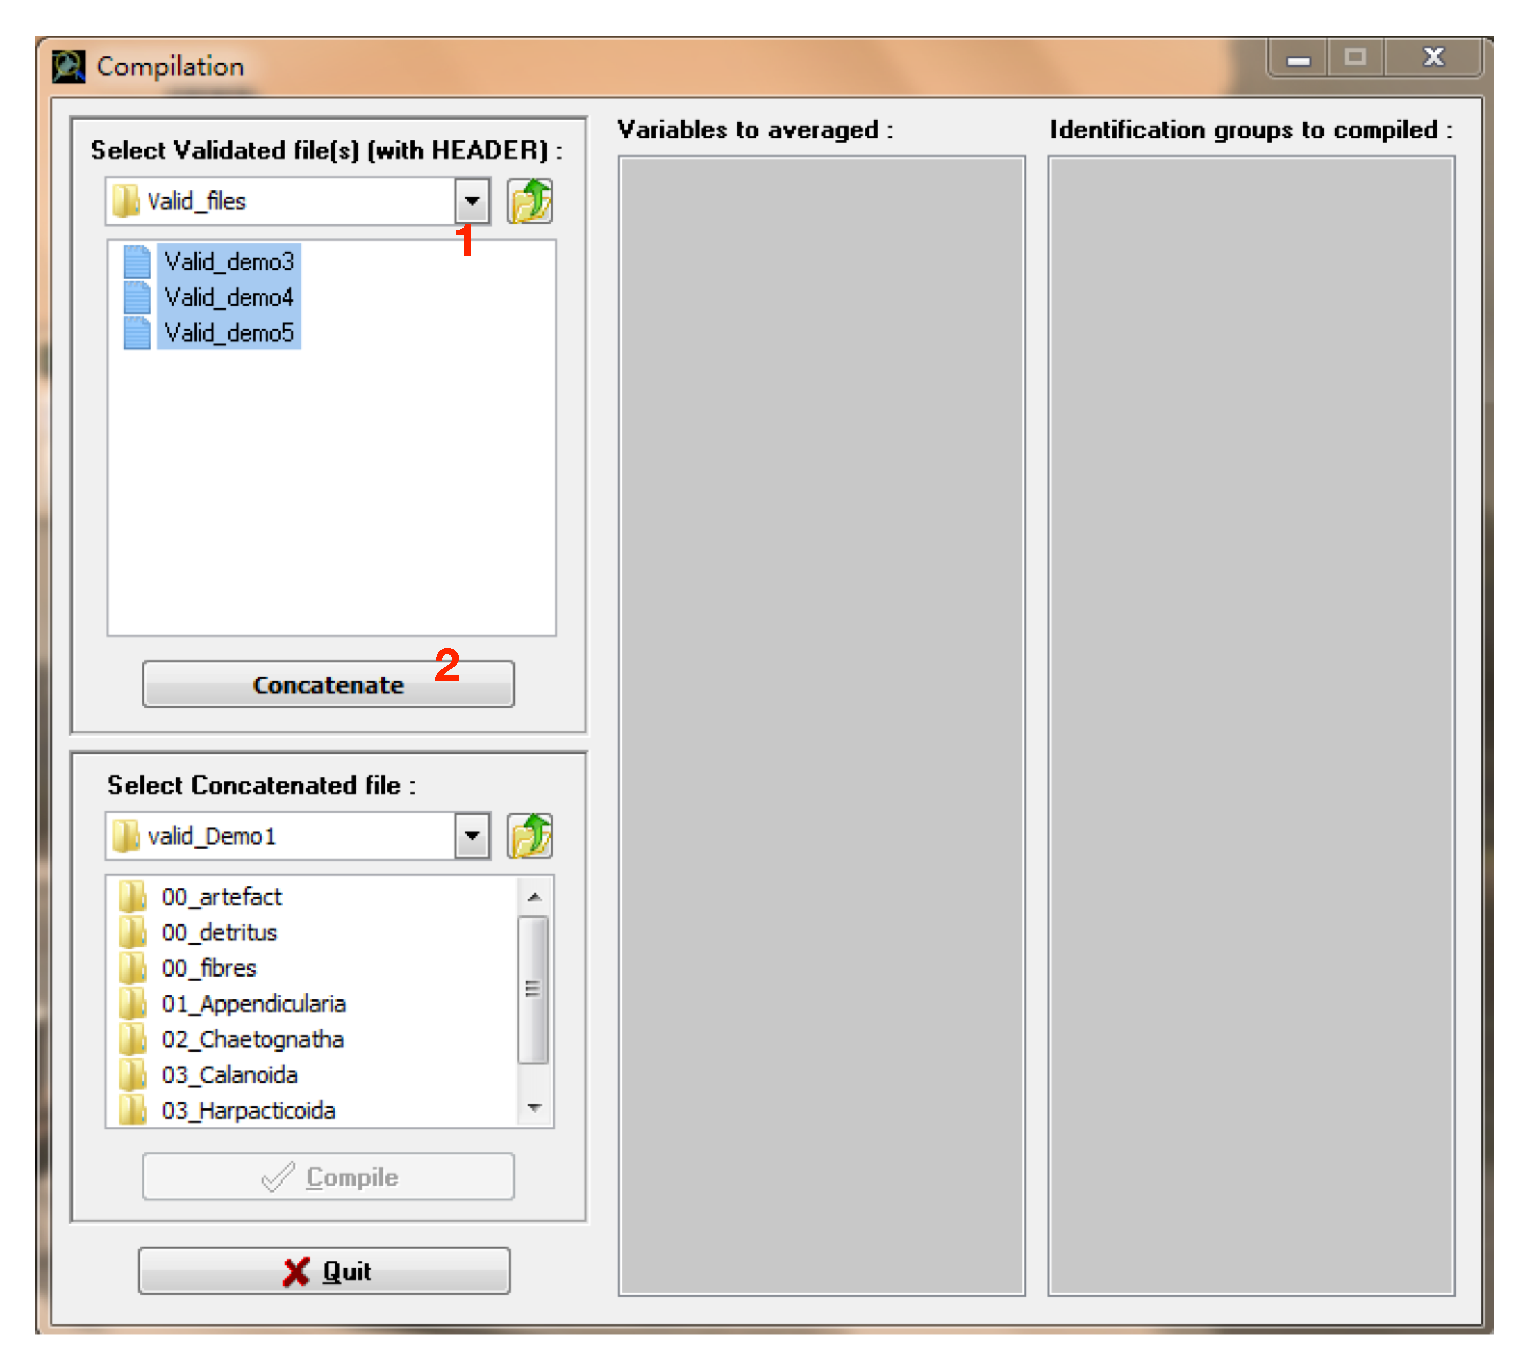
\includegraphics[width=0.7\textwidth]{CompilationWindow1.eps}
\caption{Compilation窗口:连接}
\label{fig: CompilationWindow1}
\end{figure}

1、Create a concatenation file

\begin{enumerate}
\item 浏览硬盘文件夹,找到包含你所要连接的Valid\_.txt文件的文件夹(图~\ref{fig: CompilationWindow1}: {\color{red}\textbf{1}})
\item 点击\textbf{Concatenate}(图~\ref{fig: CompilationWindow1}: {\color{red}\textbf{2}}),会出现一个保存会话框
\item 给连接后的文件进行命名,选择将其保存的文件夹路径
\item 点击\textbf{Save}按钮,连接就开始了(这可能需要几分钟,取决于你想要连接的文件数目)
\end{enumerate}

{\color{blue}\textit{注:要一次连接很多Valid\_.txt文件,需要把它们放在同一个文件夹中,然后按“Ctrl”键同时选中它们。}}

{\color{red}Create a compilation file}

\begin{figure}[!ht]
\centering
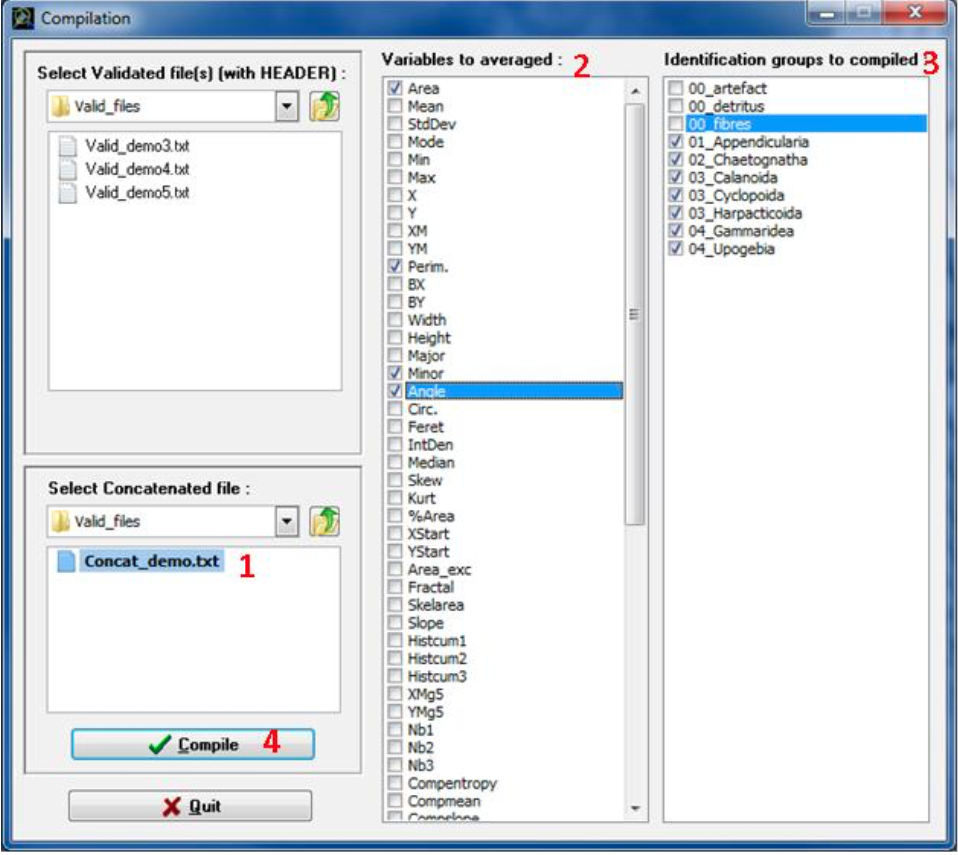
\includegraphics[width=0.7\textwidth]{CompilationWindow2}
\caption{Compilation窗口:编译}
\label{fig: CompilationWindow2}
\end{figure}

\begin{enumerate}
\item 选择一个已经连接好的Concat\_.txt文件。最终的连接文件会以粗体显示(图~\ref{fig: CompilationWindow2}: {\color{red}\textbf{1}})。
\item “Variables to averaged”一栏中可以勾选也可以不勾选相应的变量(图~\ref{fig: CompilationWindow2}: {\color{red}\textbf{2}}),被打上勾的变量在编译文件中会被平均,没有打勾的会被去除。
\item “Identification groups to compiled”一栏也可以挑选相应的类别打上勾(图~\ref{fig: CompilationWindow2}: {\color{red}\textbf{3}}),只有打上勾的类别才会计算出它所包含的物体数目。
\item 点击\textbf{Compile}按钮(图~\ref{fig: CompilationWindow2}: {\color{red}\textbf{4}}),出现一个保存会话框
\item 给编译后的文件进行命名,选择将其保存的文件夹路径
\item 点击\textbf{Save},编译就开始了
\end{enumerate}

编译后生成的文件如图~\ref{fig: CompilationFile}。

\begin{figure}[!ht]
\centering
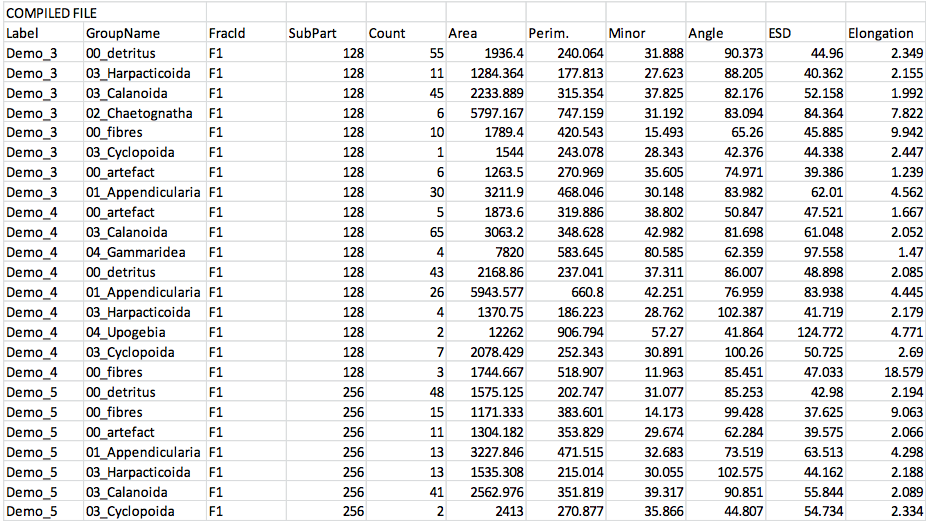
\includegraphics[width=0.7\textwidth]{CompilationFile}
\caption{编译文件}
\label{fig: CompilationFile}
\end{figure}

%\begin{enumerate}
%\item 第一列(Label):包含样本名称,按字母顺序排列
%\item 第二列(GroupNames):包含分类类别名称,按字母顺序排列
%\item 第三列(Fracld):包含
%\item 
%\item 第五列(Count):包含了每一类别的物体数目
%\item 所有被选择用来计算平均值的变量
%\end{enumerate}



\section{评价方法}

\subsection{论文中采用的评价方法}
文中采用{\color{blue}混淆矩阵(CM)}(混淆矩阵介绍见~\ref{CM})对分类器的分类效果进行评价。评价时计算的是CM的召回率(recall即the rate of true positives)和1-precision(low contamination即the rate of false positives)。

论文中的具体介绍:
\begin{tcolorbox}[colback=red!5,colframe=blue!75!black]
~~~~Evaluation of classifier performance requires the examination of a {\color{blue}Confusion matrix (CM)}, which is a contingency table crossing true (manually validated) and predicted (assigned by the classifier) identification of objects. Correct interpretation of the CM requires the examination of each category separately, including {\color{blue}the rate of true positives} as well as {\color{blue}false positives}.
\begin{itemize}
    \item the rate of true positives (recall)
        \begin{displaymath}
            true~positives=\frac{number~of~objects~correctly~predicted}{total~number~actual~objects}
        \end{displaymath}
    \item the rate of false positives (low contamination)
        \begin{displaymath}
            false~positives=\frac{number~of~objects~falsely~assigned~to~a~category}{total~number~of~predicted~objects}
        \end{displaymath}
\end{itemize}
\end{tcolorbox}

论文中的评价结果如图~\ref{fig:cmlearn}:
    \begin{figure}[!ht]
      \centering 
        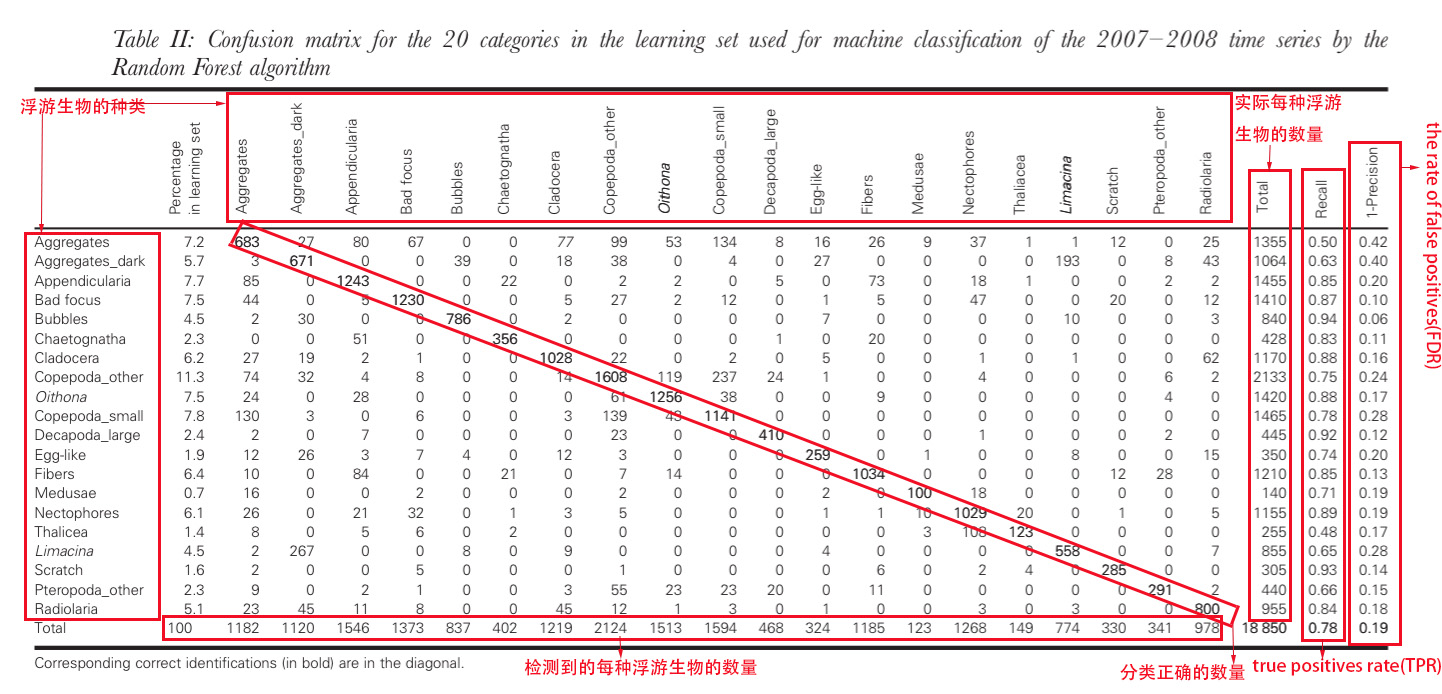
\includegraphics[width=1\textwidth]{cmlearn}
        \caption{Confusion matrix for the 20 categories in the learning set}
        \label{fig:cmlearn}
    \end{figure}
    
\subsection{怎样得到混淆矩阵}
论文中提到三种得到CM的方法(即采用什么训练集和测试集来生成):
    \begin{enumerate}
        \item Re-substitution CM
        
       这个方法是采用的测试集和训练集为同一个数据集。在这个过程中,用产生的分类器对测试集进分类时,得到的分类结果错误较少甚至可能没有错误,采用CM进行评价时就会低估分类器的错误率。
        \item Cross-validation CM
        
        这个方法是采用交叉验证(交叉验证介绍见\ref{cv})的方法。在这个过程中,将一个数据集分成n个相等的子集,用其中n-1个子集来训练产生分类器,用剩下的1个子集来进行测试,重复进行n次来构建CM。
        \item Uses two equivalent and independent learning files describing the same categories with different objects
        
        这种方法是用两个相等且相互独立的数据集分别作为训练集和测试集,根据测试结果建立CM。两个相等的数据集即在两个集合中浮游生物的种类相同,但是每种浮游生物中的个体是不同的。
    \end{enumerate}
    
\subsection{PkID中的评价参数}
PkID中通过5-折交叉验证 (介绍见\ref{kCM}) 得到混淆矩阵,对分类器进行评价。5-折交叉验证将数 据集分为 5 份,轮流将其中 4 份作为训练数据,1 份作为测试数据,进行试验。每次试验都会得出相 应的误分类率 (error rate 介绍见\ref{kCM}) 如图\ref{fig:five}。
    \begin{figure}[!ht]
      \centering 
        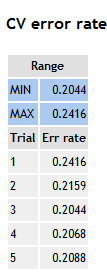
\includegraphics[width=0.1\textwidth]{five}
        \caption{5 次的误分类率}
        \label{fig:five}
    \end{figure}
    
    交叉验证得到的分类器总混淆矩阵(五次分类的累计结果)和误分类率(五次分类误分类率的平均值)如图\ref{fig:pkidCM}。
   \begin{figure}[!ht]
      \centering 
        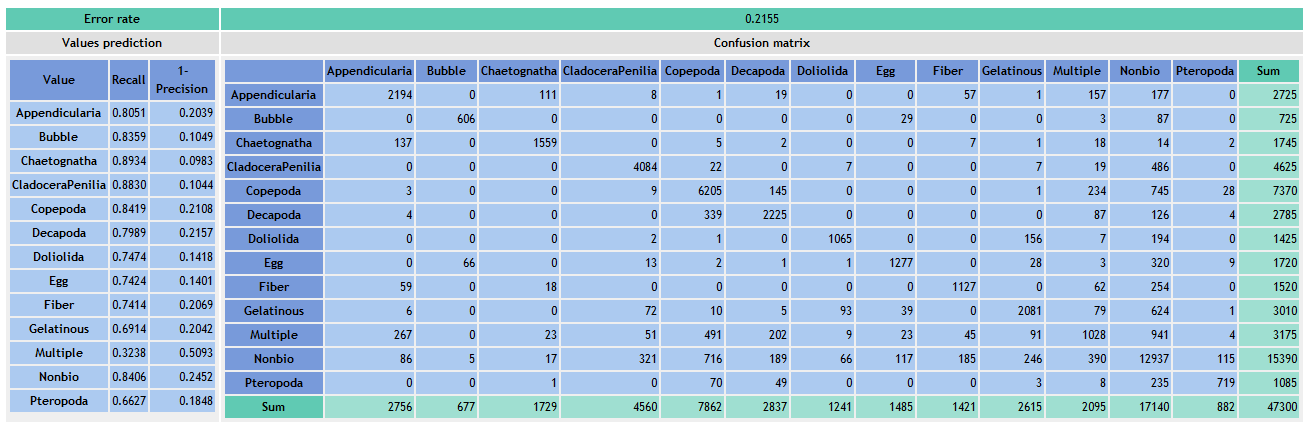
\includegraphics[width=1\textwidth]{pkidCM}
        \caption{交叉验证得到的总混淆矩阵和误分类率}
        \label{fig:pkidCM}
    \end{figure}
    

%    \begin{tcolorbox}[colback=red!5,colframe=blue!75!black]
%    There are three ways to build a CM, all available in PkID.
%    \end{tcolorbox}
    



\subsection{混淆矩阵Confusion matrix (CM)}
\label{CM}

在机器学习中,混淆矩阵(CM)是一种比较简单的对学习算法性能进行评价的评估准则,而且是大多数指标的基础。常用的算法评估准则有:Confusion Matrix、ROC、Lift、Gini、K-S等等。\newline

混淆矩阵 (CM)\footnote{\url{http://baike.baidu.com/view/2781781.htm}}\footnote{\url{http://en.wikipedia.org/wiki/Confusion_matrix}}:混淆矩阵是一种评估分类器可信度的方法。在图像精度评价中,主要用于比较分类结果和实际测得值,可以把分类结果的精度显示在一个混淆矩阵里面。特别用于监督学习,在无监督学习一般叫做匹配矩阵。

混淆矩阵是一个n行n列的矩阵,n代表类别的数量。矩阵的每一列代表预测的每一类的数量,每一行代表实际的每一类的数量。对角线上表示分类正确的每一类的数量。

例如:有150个样本数据,这些数据实际分为3类,每类50个。分类结束后得到的混淆矩阵如图\ref{fig:cm}。例如:第一行说明类1的50个样本有43个样本分类正确,5个错分为类2,2个错分为类3;第一列说明类1有43个样本分类正确,类2的2个样本被错分为类1,类3没有样本被错分为类1;对角线上的数据表示,类1、2、3分别有43、45、49个样本被分类正确。\newline
    \begin{figure}[!ht]
      \centering 
        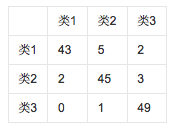
\includegraphics[width=0.3\textwidth]{cm}
        \caption{混淆矩阵例子}
        \label{fig:cm}
    \end{figure}

根据混淆矩阵可以导出以下几个参数\footnote{\url{http://www2.cs.uregina.ca/~dbd/cs831/notes/confusion_matrix/confusion_matrix.html}}:
\begin{itemize}
    \item true positives (TP):正样本被识别出的数量
    \item true negatives (TN):负样本被识别出的数量
    \item false positives (FP):负样本被错误分为正样本的数量
    \item false negatives (FN):正样本被错误分为负样本的数量\newline
    
    \item Accuracy:准确率,针对分类器的整个预测情况。
        \begin{displaymath}
            Accuracy=\frac{TP+TN}{TP+TN+FP+FN}
        \end{displaymath}
    \item {\color{red}Error rate:误分类率,针对分类器的整体预测情况。}(PkID 中使用的评价参数)
        \begin{displaymath}
            Error rate=\frac{FP+FN}{TP+TN+FP+FN}
        \end{displaymath}
    \item {\color{blue}The true positive rate (TPR) :召回率,就是正样本被识别出的概率。}(文中和PkID中使用的评价参数)
        \begin{displaymath}
            TPR=\frac{TP}{TP+FN}
        \end{displaymath}
     \item The false positive rate (FPR):虚警率,负样本被错误分为正样本的概率。
        \begin{displaymath}
            FPR=\frac{FP}{FP+TN}
        \end{displaymath}
    \item The true negative rate (TNR):负样本被识别出的概率
        \begin{displaymath}
            TNR=\frac{TN}{FP+TN}
        \end{displaymath}

    \item The false negative rate (FNR) :漏警率,正样本被错误分为负样本的概率。
        \begin{displaymath}
            FNR=\frac{FN}{FN+TP}
        \end{displaymath}
    \item {\color{blue}False discovery rate (FDR):1-precision。}(文中和 PkID 中使用的评价参数)
        \begin{displaymath}
            FDR=\frac{FP}{FP+TP}
        \end{displaymath}
    \item Positive predictive value (PPV)
        \begin{displaymath}
            PPV=\frac{TP}{TP+FP}
        \end{displaymath}
    \item Negative predictive value (NPV)
        \begin{displaymath}
            NPV=\frac{TN}{TN+FN}
        \end{displaymath}
    
\end{itemize}

\begin{figure}[!ht]
\centering
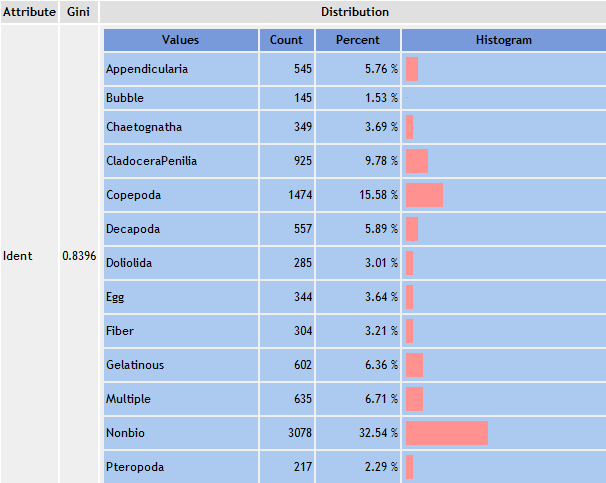
\includegraphics[width=0.8\textwidth]{每个类别所占比例.png}
\caption{数据集中每种类别的数目及所占比例}
\label{fig: ratio}
\end{figure} 

\subsection{交叉验证Cross Validation (CV)}
\label{cv}
交叉验证是用来验证分类器的性能一种统计分析方法,基本思想是把在某种意义下将原始数据进行分组,一部分做为训练集(training set),另一部分做为验证集(validation set),首先用训练集对分类器进行训练,在利用验证集来测试训练得到的模型,以此来做为评价分类器的性能指标。
\subsubsection{训练集和测试集}

在模式识别与机器学习的相关研究中,经常会将数据集分为训练集跟测试集这两个子集,前者用以建立模型,后者则用来评估该模型对未知样本进行预测时的精确度,正规的说法是泛化能力。怎么将完整的数据集分为训练集跟测试集,必须遵守如下要点:
\begin{enumerate}
    \item 只有训练集才可以用在模型的训练过程中,测试集则必须在模型完成之后才被用来评估模型优劣的依据。
    \item 训练集中样本数量必须够多,一般至少大于总样本数的50\%。
    \item 两组子集必须从完整集合中均匀取样。
\end{enumerate}

        {\color{blue}注:}其中最后一点特别重要,均匀取样的目的是希望减少训练集和测试集与完整集合之间的偏差,但却也不易做到。一般的作法是随机取样,当样本数量足够时,便可达到均匀取样的效果,然而随机也正是此作法的盲点,也是经常是可以在数据上做手脚的地方。举例来说,当辨识率不理想时,便重新取样一组训练集和测试集,直到测试集的识别率满意为止,但严格来说这样便算是作弊了。
        
        在MATALB中使用cvpartition对数据集进行随机拆分,完成交叉验证。
        
\subsubsection{常见的交叉验证方法}

\begin{itemize}
    \item Hold-Out Method
    
    将原始数据随机分为两组,一组做为训练集,一组做为验证集。
    \item Double Cross Validation(2-fold Cross Validation,记为2-CV)
    
    将数据集分成两个相等大小的子集,进行两回合的分类器训练。在第一回合中,一个子集作为training set,另一个便作为testing set;在第二回合中,则将training set与testing set对换后,再次训练分类器。
    {\color{blue}\item K-fold Cross Validation(K-折交叉验证,记为K-CV)}(实验中采用的交叉验证方法)
    \label{kCM}
    将原始数据分成K组,将每个子集数据分别做一次验证集,其余的K-1组子集数据作为训练集,这样会得到K个模型,用这K个模型最终的验证集的分类准确率的平均数作为此K-CV下分类器的性能指标。K一般大于等于2,实际操作时一般从3开始取。
    \item Leave-One-Out Cross Validation(记为LOO-CV)
    
    将每个样本单独作为验证集,其余的N-1个样本作为训练集,所以LOO-CV会得到N个模型,用这N个模型最终的验证集的分类准确率的平均数作为此下LOO-CV分类器的性能指标。相比于前面的K-CV,LOO-CV有两个明显的优点:
    \begin{itemize}
        \item 每一回合中几乎所有的样本皆用于训练模型,因此最接近原始样本的分布,这样评估所得的结果比较可靠。
        \item 实验过程中没有随机因素会影响实验数据,确保实验过程是可以被复制的。
    \end{itemize}
\end{itemize}


\section{特征(PkID)}

PkID中用到的特征一共有67个:Area, Mean, StdDev, Mode, Min, Max, X, Y, XM, YM, Perim., BX, BY, Width, Height, Major, Minor, Angle, Circ., Feret, IntDen, Median, Skew, Kurt, \%Area, XStart, YStart, Area\_exc, Fractal, Skelarea, Slope, Histcum1, Histcum2, Histcum3, XMg5, YMg5, Nb1, Nb2, Nb3, Compentropy, Compmean, Compslope, CompM1, CompM2, CompM3, Symetrieh, Symetriev, Symetriehc, Symetrievc, Convperim, Convarea, Fcons, ThickR, Tag, ESD, Elongation, Range, MeanPos, CentroidsD, CV, SR, PerimAreaexc, FeretAreaexc, PerimFeret, PerimMaj, Circexc, CDexc

从训练集的PID文件文件中看到,Compentropy, Compmean, Compslope, CompM1, CompM2, CompM3这6个特征在所有图像上的值都为0,在训练分类器时是不起作用的。这6个特征的具体含义也没有找到。

\subsection{位置特征}

\begin{description}
\item[BX] 能够包围物体,且平行于图像两条边的最小外界矩形的左上角顶点的X坐标 
\item[BY] 能够包围物体,且平行于图像两条边的最小外界矩形的左上角顶点的Y坐标 
\item[Height] 能够包围物体,且平行于图像两条边的最小外界矩形的高
\item[Width] 能够包围物体,且平行于图像两条边的最小外界矩形的宽
\item[XStart] 图像最左上角像素点的X坐标
\item[YStart] 图像最左上角像素点的Y坐标
\item[XM] 物体灰度重心的X坐标
\item[YM] 物体灰度重心的Y坐标
\item[XMg5] gamma值为51时的物体灰度重心的X坐标
\item[YMg5] gamma值为51时的物体灰度重心的Y坐标
\item[X] 物体重心点的X坐标
\item[Y] 物体重心点的Y坐标
\end{description}

\subsection{尺寸特征}

\begin{description}
\item[Area] 包含物体的最小矩形面积 
\item[Perim] 物体最外层边缘的长度
\item[Major] 物体内切椭圆的长轴
\item[Minor] 物体内切椭圆的短轴
\item[Feret] Maximum feret diameter(最大费雷特径), 沿物体边缘任意两个点的最长距离
\item[Area\_exc] 去掉物体空洞后的表面积,空洞是指灰度值与背景相同的部分
\item[\%area] 物体表面积中空洞所占的百分比,即背景所占的比例
\end{description}

\subsection{灰度值特征}

\begin{description}
\item[Min] 物体内部所有像素点的最小灰度值 (0 = black)
\item[Max] 物体内部所有像素点的最大灰度值 (255 = white)
\item[Mean] 物体内的平均灰度值; 物体中所有像素点的灰度值的总和除以总的像素个数
\item[IntDen] Integrated density(总密度)。物体内像素点的灰度值的总和($IntDen = Area * Mean$)
\item[StdDev] 物体内像素的灰度值的标准差
\item[Mode] Modal grey value within the object
\item[Skew] 灰度直方图的偏斜度,是灰度分布是否符合正态分布的检验参数
\item[Kurt] 灰度直方图的峰值 
\item[Mean\_exc] 物体内部去掉空洞后的平均灰度值 ($Mean\_exc = IntDen / Area\_exc$)
\item[Median] 物体内像素的灰度值的中位数
\item[Slope] 归一化的灰度累计直方图的斜率
\item[Histcum1] 灰度累计直方图的值为25\%时所对应的灰度值
\item[Histcum2] 灰度累计直方图的值为50\%时所对应的灰度值
\item[Histcum3] 灰度累计直方图的值为75\%时所对应的灰度值
\end{description}

\subsection{形状特征}

\begin{description}
\item[Fractal] 物体边界的分形维数 (Berube and Jebrak, 1999),表明物体边界的不规则程度
\item[Skelarea] 骨架像素的表面积(在二值图像中,不断地从物体边缘处减去像素点直到仅剩一个像素的宽度,最后所得图形的像素点数)
\item[Circ] $Circularity = (4 * Pi * Area) / Perim^2$; 表征物体接近圆的程度,值等于1时,说明物体为正圆形,值越接近0,物体体形越长。
\item[Angle] 浮游动物主轴与图片x轴形成的夹角,在图片切割后旋转图片测量相关参数使用
\item[Symetrieh] 水平对称
\item[Symetriev] 垂直对称
\item[Symetriehc]
\item[Symetrievc]
\end{description}

\subsection{自定义特征}

\begin{description}
    \item[ESD] $2 \times \sqrt{\cfrac{Area}{\pi}}$
    \item[Elongation] $\cfrac{Major}{Minor}$
    \item[Range] $Max-Min$
    \item[MeanPos] $\cfrac{Mean-Max}{Max-Min}$
    \item[CentrodisD] $\sqrt{(XM-X)^{2}+(YM-Y)^{2}}$
    \item[CV] $100 \times \cfrac{StdDev}{Mean}$
    \item[SR] $100 \times \cfrac{StdDev}{Max-Min}$
    \item[PerimAreaexc] $\cfrac{Perim}{\sqrt{Area\_exc}}$
    \item[FeretAreaexc] $\cfrac{Feret}{\sqrt{Area\_exc}}$
    \item[PerimFeret] $\cfrac{Perim}{Feret}$
    \item[PerimMaj] $\cfrac{Perim}{Major}$
    \item[Circexc] $\cfrac{4 \times \pi Area\_exc}{Perim^{2}}$
    \item[CDexc] $\cfrac{\sqrt{(XM-X)^{2}+(YM-Y)^{2}}}{{\sqrt{Area\_exc}}}$
\end{description}


\section{识别结果分析}

采用交叉验证的方法来评价分类器的性能好坏,所选用的数据集中的类别如图~\ref{fig: ratio}所示,其中有10个是浮游动物类,包括Appendicularia(被囊类)、Chaetognatha(毛颚类)、CladoceraPenilia(枝角类喙)、Copepoda(桡足类)、Decapoda(十足类)、Doliolida(海樽类)、Egg(蛋类)、Pteropoda(翼足类)、Gelatinous(凝胶纤维)、Multiple。3个非浮游动物类:Nonbio(非生物类)、Bubble(气泡)、Fiber(纤维)。将该数据集随机均分为$n$份,其中每个子集数据分别做一次验证集,其余的$n-1$组子集数据作为训练集,这样会得到$n$个模型,用这$n$个模型最终的验证集的分类准确率的平均数作为此分类器的性能指标。

采用随机森林学习算法,67个特征的评价结果如图~\ref{fig: RandomForest}。

\begin{figure}[!ht]
\centering
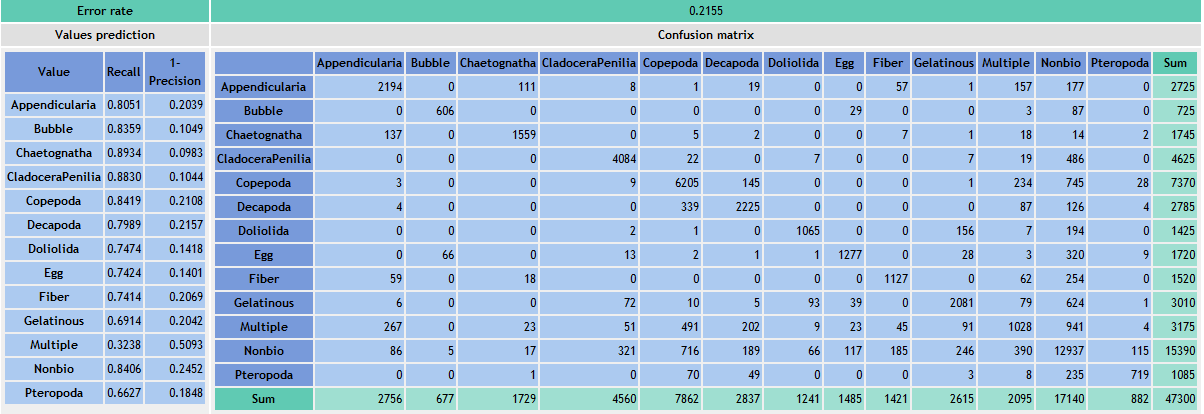
\includegraphics[width=1.0\textwidth]{RandomForest.png}
\caption{Random Forest}
\label{fig: RandomForest}
\end{figure} 

采用随机森林算法,去掉以下位置特征(XM, YM, BX, BY, Width, Height, Angle, XStart, YStart, XMg5, YMg5, X, Y)的评价结果如图~\ref{fig: withoutposition},可以看到,与用所有特征相比,去除不必要的位置特征会使评价结果有所提高,对所有种类的Recall值、Precision值求平均(除了Multi类),得到的平均的Recall值为0.799,平均的Precision值为0.161。PID文件中的位置特征大多是ImageJ自带的,是用来生成缩略图所需的参数,在训练分类器时并没有使用。

\begin{figure}[!ht]
\centering
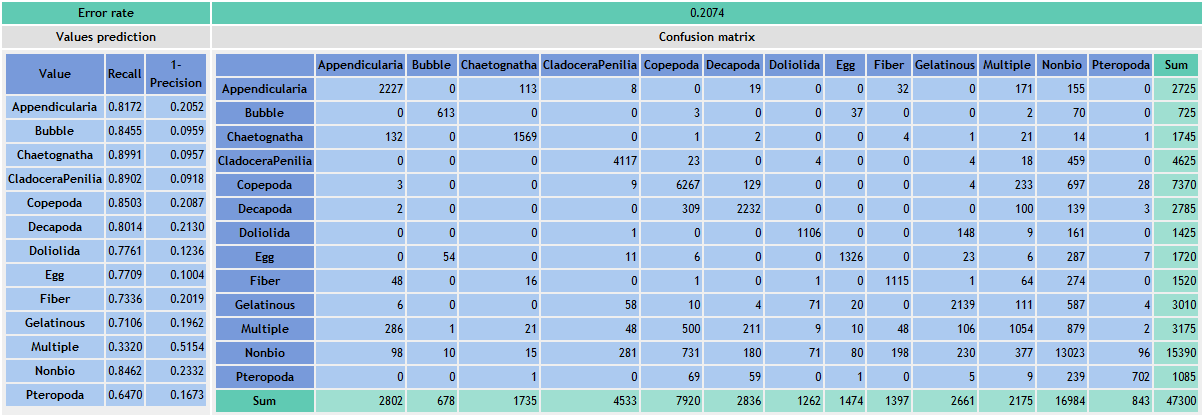
\includegraphics[width=1.0\textwidth]{withoutposition.png}
\caption{Random Forest (without position variables)}
\label{fig: withoutposition}
\end{figure} 

采用K-NN算法,去掉位置特征后的评价结果如图~\ref{fig: KNN}。

\begin{figure}[!ht]
\centering
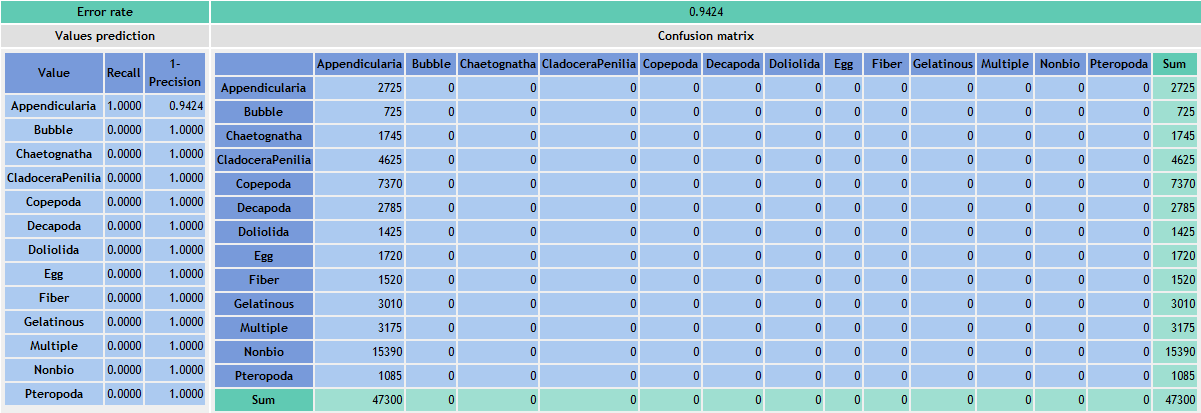
\includegraphics[width=1.0\textwidth]{KNN.png}
\caption{K-NN (without position variables)}
\label{fig: KNN}
\end{figure} 

采用C-SVC linear算法,去掉位置特征后的评价结果如图~\ref{fig: C-SVClinear}。

\begin{figure}[!ht]
\centering
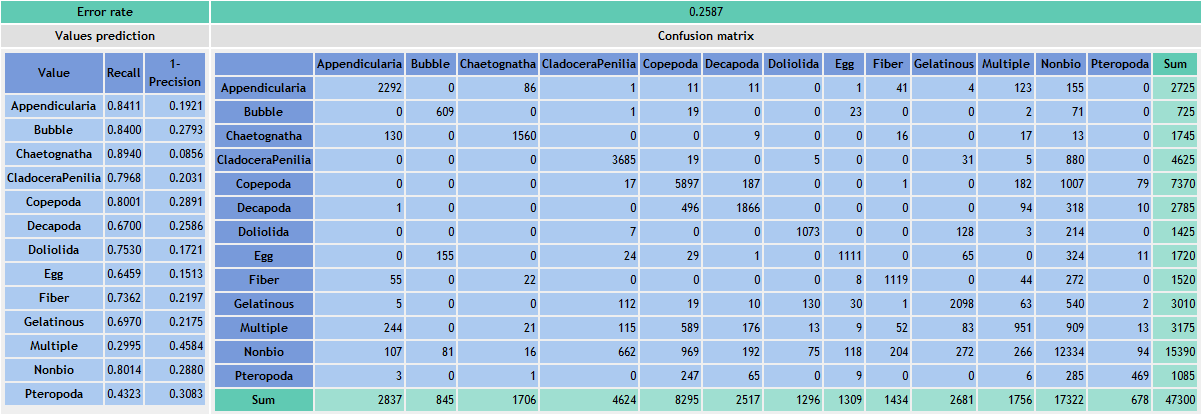
\includegraphics[width=1.0\textwidth]{C-SVClinear.png}
\caption{C-SVC linear (without position variables)}
\label{fig: C-SVClinear}
\end{figure} 

采用C-SVC RBF算法,去掉位置特征后的评价结果如图~\ref{fig: C-SVC-RBF}。

\begin{figure}[!ht]
\centering
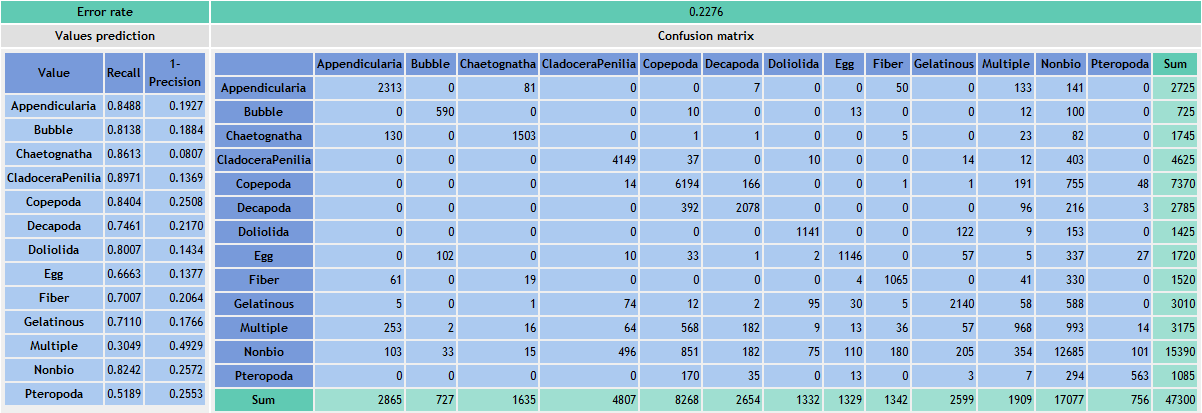
\includegraphics[width=1.0\textwidth]{C-SVC-RBF.png}
\caption{C-SVC RBF (without position variables)}
\label{fig: C-SVC-RBF}
\end{figure} 

采用BVM RBF算法,去掉位置特征后的评价结果如图~\ref{fig: BVM-RBF}。

\begin{figure}[!ht]
\centering
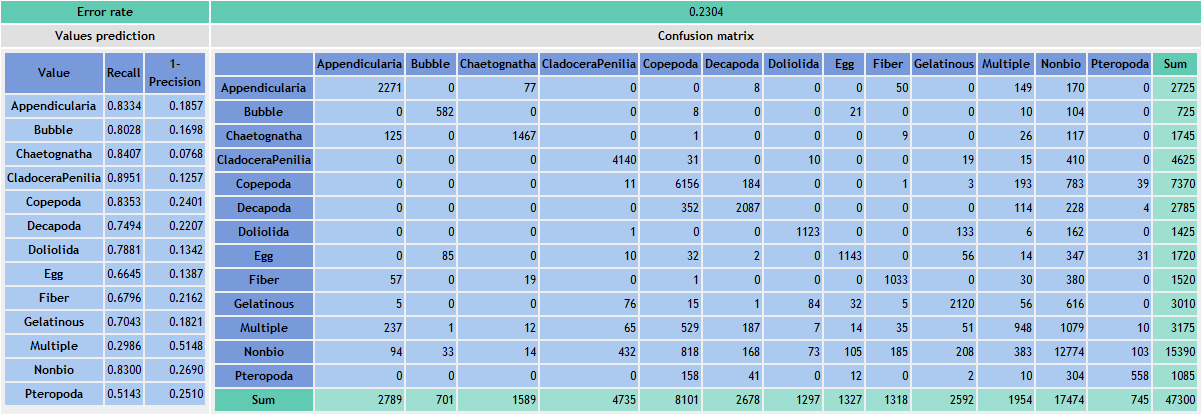
\includegraphics[width=1.0\textwidth]{BVM-RBF.png}
\caption{BVM RBF (without position variables)}
\label{fig: BVM-RBF}
\end{figure} 

采用PLS算法,去掉位置特征后的评价结果如图~\ref{fig: PLS}。

\begin{figure}[!ht]
\centering
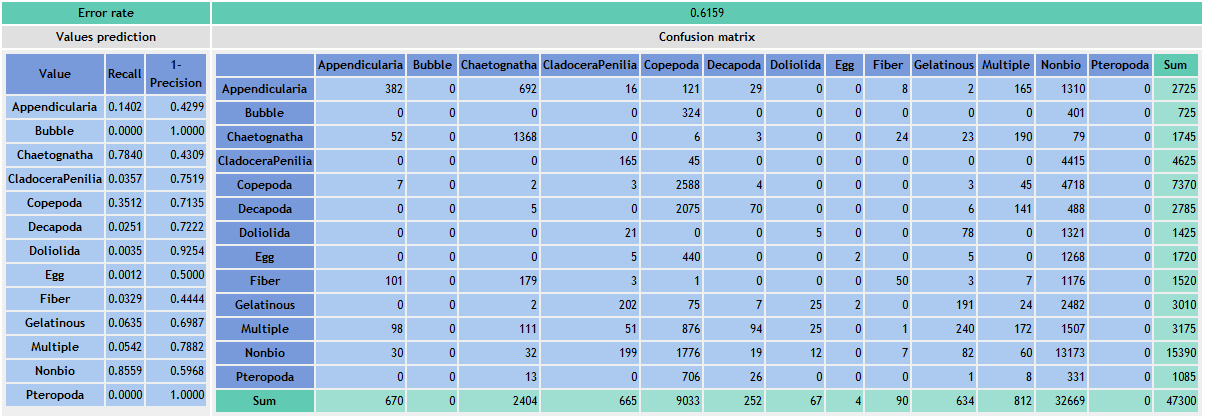
\includegraphics[width=1.0\textwidth]{PLS.png}
\caption{PLS (without position variables)}
\label{fig: PLS}
\end{figure} 

采用Multilayer perceptron算法,去掉位置特征后的评价结果如图~\ref{fig: MultilayerPerceptron}。

\begin{figure}[!ht]
\centering
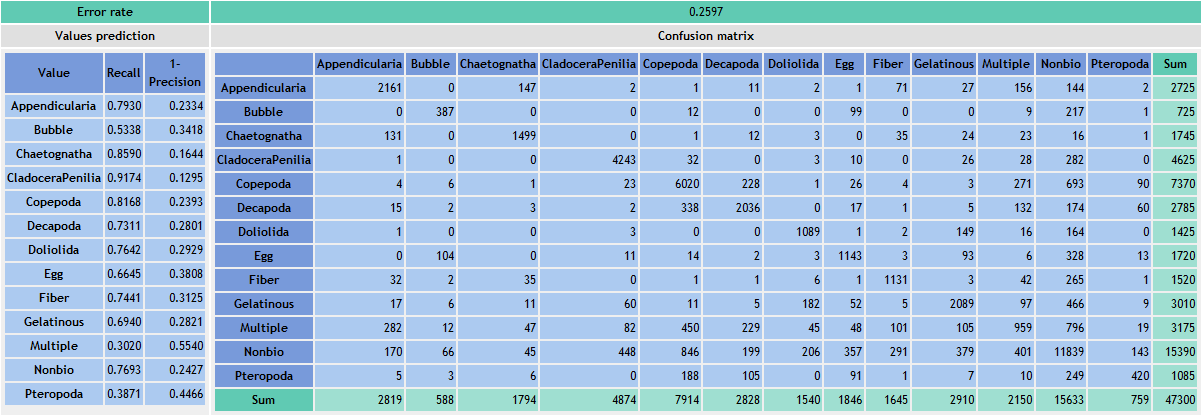
\includegraphics[width=1.0\textwidth]{MultilayerPerceptron.png}
\caption{MultilayerPerceptron (without position variables)}
\label{fig: MultilayerPerceptron}
\end{figure} 

\section{优缺点分析}

PkID主要用了灰度特征、尺寸特征和形状特征。其中灰度特征跟灰度图的质量有很大关系,并不能完全准确地将不同种类区分开来,这里可以尝试加入一些灰度对比度特征。对于尺寸特征,每幅图像中都有一个5mm的标尺,可以依据标尺来度量物体的一些长度特征。人在进行浮游动物分类时,主要是依据形状特征,所以形状特征应该是最重要的,但PkID中只采用了少数简单的形状特征,因而不能充分地表示某一类浮游动物。

对于具体哪些特征是有用的哪些是没用的,还得通过具体的实验才能看出来。单从缩略图来看,这三类特征都是有用的,都有区分作用,但是还不充足,还应该再加入一些更合理的特征。

\section{特征(Ours)}

\subsection{经典特征}

\subsubsection{HOG特征}

HOG\cite{dalal2005histograms}(Histogram of oriented gradients,方向梯度直方图)是一种在计算机视觉和图像处理中用来进行物体检测的特征描述子,它通过统计图像局部区域的梯度方向直方图来构成特征。Hog特征结合\textbf{SVM分类器}已经被广泛应用于图像识别中,尤其在\textbf{行人检测}中获得了极大的成功。

{\color{blue}主要思想}:局部目标的表象和形状能够被梯度或边缘的方向密度分布很好地描述。
%首先计算图片中不同方向上的梯度值,然后将图像分成小的连通区域,我们把它叫细胞单元(cell),采集细胞单元中各像素点的梯度或边缘的方向直方图,这个直方图就可以代表这块区域的特征。

{\color{blue}具体实现方法}:将图像分成小的连通区域,我们把它叫细胞单元(cell)。然后采集细胞单元中各像素点的梯度的或边缘的方向直方图,最后把这些直方图组合起来就可以构成特征描述器。具体实现流程如图\ref{fig:shixian}。
        \begin{figure}
            \centering
            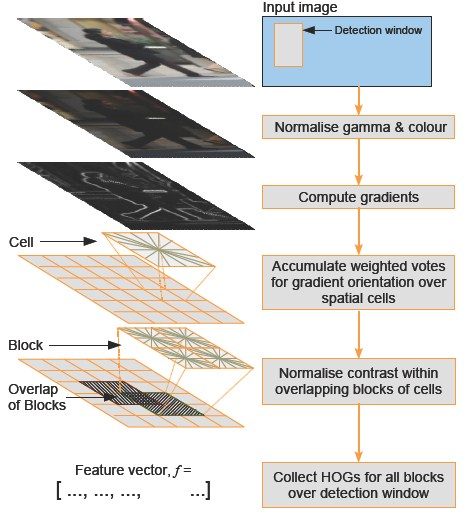
\includegraphics[width=0.4\linewidth]{flowchart}
            \caption{HOG特征}
            \label{fig:shixian}
        \end{figure}

{\color{blue}算法步骤}:

(1)图像归一化。采用 Gamma 校正法对输入图像进行颜色空间的标准化 ;目的是调节图像的对比度,降低图像局部的阴影和光照变化所造成的影响,同时可以抑制噪音的干扰。

Gamma压缩公式:
\begin{displaymath}
    I(x,y)=I(x,y)^{gamma}
\end{displaymath}

比如可以取Gamma=$\frac{1}{2}$。

(2)利用一阶微分计算每一个像素的梯度(包括大小和方向);目的是为了捕获轮廓信息,同时进一步弱化光照的干扰。
    
    采用模板$[-1~0~1]$(实验表明采用模板$[-1~0~1]$求得的梯度效果最好)计算水平和垂直方向的梯度:
        \begin{displaymath}
        G_{h}(x,y)=f(x+1,y)-f(x-1,y)~~~~\forall x,y
        \end{displaymath}
        \begin{displaymath}
        G_{v}(x,y)=f(x,y+1)-f(x,y-1)~~~~\forall x,y
        \end{displaymath}
        
        计算梯度值和梯度方向:
        \begin{displaymath}
        M(x,y)=\sqrt{G_{h}(x,y)^{2}+G_{v}(x,y)^2}
        \end{displaymath}
        \begin{displaymath}
        \theta(x,y)=\arctan\frac{G_{h}(x,y)}{G_{v}(x,y)}
        \end{displaymath}
        
(3)将图像划分成小cells(例如$6 \times 6$像素/cell)。

(4)统计每个cell的梯度直方图,可形成每个cell的描述子;
        
        构建每个单元的梯度方向直方图,将cell的梯度方向360度根据需要分成m个bin,例如图\ref{fig:bin}分成了16个bin。然后根据每个像素点的梯度方向,采用加权投票的方式得到直方图,即每一票都是带权值的,这个权值是根据该像素点的梯度幅度计算出来的。
        \begin{figure}
            \centering
            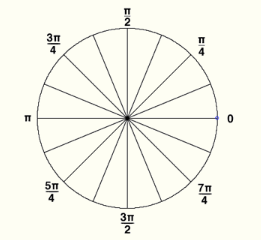
\includegraphics[width=0.3\linewidth]{bin}
            \caption{梯度方向bin}
            \label{fig:bin}
        \end{figure}
       % 一张图像由若干个块(Block)组成,一个块(Block)都由若干单元(Cell)组成,一个单元都有若干个像素点组成。块与单元的关系如图\ref{fig:block}。
       
(5)将每几个cell组成一个块(block)(例如$3 \times 3 $个cell/block),一个block内所有cell的梯度直方图串联起来便得到该block的HOG特征描述子。
    
    把各个细胞单元组合成大的、空间上连通的区间(blocks)。这样以来,HOG描述器就变成了由各区间所有细胞单元的直方图成分所组成的一个向量。这些区间是互有重叠的,这就意味着:每一个细胞单元的输出都多次作用于最终的描述器。区间有两个主要的几何形状——矩形区间(R-HOG)和环形区间(C-HOG)如图\ref{fig:shape}。
        \begin{figure}
            \centering
            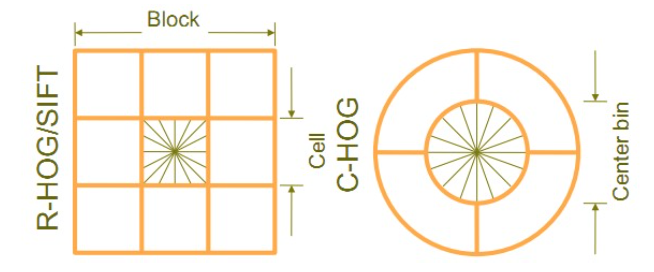
\includegraphics[width=0.5\linewidth]{shape}
            \caption{矩形区间和环形区间}
            \label{fig:shape}
        \end{figure}
        
(6)将图像内的所有block的HOG特征直方图串联起来就可以得到该图像的HOG特征描述子了。这个就是最终的可供分类使用的特征向量了。
    \begin{comment}
    对block块内特征向量的归一化主要是为了使特征向量空间对光照,阴影和边缘变化具有鲁棒性。作者采用了四中不同的方法对区间进行归一化,并对结果进行了比较。引入$v$表示一个还没有被归一化的向量,它包含了给定区间(block)的所有直方图信息。$||v_{k}||$表示v的k阶范数,这里的$k$为1、2。用$\varepsilon$表示一个很小的常数。这时,归一化因子可以表示如下:
    \begin{displaymath}
    L_{2}-norm, v \gets \frac{v}{\sqrt{||v||_{2}^{2}+\varepsilon^{2}}}
    \end{displaymath}
    \begin{displaymath}
    L_{2}-Hys% $(方法同上,只是限制v的最大值到0.2,然后再次重新标准化)$
    \end{displaymath}
    \begin{displaymath}
    L_{1}-norm, v \gets \frac{v}{||v||_{1}+\varepsilon}
    \end{displaymath}
    \begin{displaymath}
    L_{1}-sqrt, v \gets \frac{v}{\sqrt{||v||_{1}+\varepsilon}}
    \end{displaymath}
    \end{comment}

    最终可以得到一个$m \times n \times \alpha$个数据组成的高维向量,其中$m$表示每个cell中方向bin的数目,$n,\alpha$分别表示block的个数以及一个block中cell的数目。

{\color{blue}在行人检测中的应用}:

用一个窗口(OpenCV采用$64 \times 128$)在图像中滑动,计算窗口对应的hog特征。窗口中块的大小为$16 \times 16$,块的步长为$8 \times 8$,单元的大小为$8 \times 8$。把每一个胞元投影到9个bin,那么每一个单元对应的向量就是9维,每个bin对应该9维向量的一个数。该窗口特征向量的维数为:$9 \times \frac{16}{8} \times \frac{16}{8} \times (\frac{64-16}{8}+1) \times (\frac{128-16}{8}+1)=3780$。

{\color{blue}代码}:

采用vl\_feat中的hog特征函数:
    \begin{lstlisting}[language=C++]
    hog = vl_hog(img, cellsize);//img表示输入的图像,cellsize为单元的大小
    image = vl_hog('render', hog);//将hog特征转换为图像
    \end{lstlisting}

\subsubsection{SIFT特征}

SIFT(Scale invariant feature transform,尺度不变特征变换)是一种检测局部特征的算法,该算法通过求得一幅图像中的特征点及有关尺度和方向的描述子得到特征并进行图像特征点匹配,它由 David Lowe 在 1999 年\cite{lowe1999object}所发表, 2004 年\cite{lowe2004distinctive}完善总结。%SIFT算法提取的特征点具有尺度不变性,也就是说,同一物体在图像上不论尺度大小,都能根据SIFT算法提取到相同的特征点。

{\color{blue}主要思想}:SIFT算法是一种提取局部特征的算法,在尺度空间寻找极值点,提取位置、尺度、旋转不变量。

{\color{blue}算法步骤}:

(1)构建尺度空间,检测极值点,获得尺度不变性。
    
    通过高斯微分函数来识别潜在的对于尺度和旋转不变的兴趣点。用不同尺度(标准差)的高斯函数对图像进行平滑,然后比较平滑后图像的差别,差别大的像素就是特征明显的点。
    
    原始图像经过不同尺度的高斯模糊所得的一组图像空间定义为:
    \begin{displaymath}
        L(x,y,\sigma)=G(x,y,\sigma)*I(x,y)
    \end{displaymath}
    
    其中$I(x,y)$是原始图像,$\sigma$大小决定图像的平滑程度,$G(x,y,\sigma)$是尺度可变高斯函数:
    \begin{displaymath}
        G(x,y,\sigma)=\frac{1}{2\pi \sigma^{2}}e^{\frac{-(x^{2}+y^{2})}{2\sigma^{2}}}
    \end{displaymath}
    
    为了有效地在尺度空间检测到稳定的关键点,提出了高斯差分尺度空间。利用 不同尺度的高斯差分核与图像卷积生成。
    \begin{displaymath}
        D(x,y,\sigma)=[G(x,y,k\sigma)-G(x,y,\sigma)]*I(x,y)=L(x,y,k\sigma)-L(x,y,\sigma)
    \end{displaymath}
    
(2)精确定位出特征关键点的位置。

(3)为关键点指定方向参数。

利用关键点邻域像素的梯度方向分布特性,我们可以为每个关键点指定方向参数方向,从而使描述子对图像旋转具有不变性,我们通过求每个极值点的梯度来为极值点赋予方向。
\begin{displaymath}
    m(x,y)=\sqrt{[L(x+1,y)-L(x-1,y)^{2}+[L(x,y+1)-L(x,y-1)]^{2}]}
\end{displaymath}
\begin{displaymath}
    \theta(x,y)=\alpha\tan2\frac{L(x,y+1)-L(x,y-1)}{L(x+1,y)-L(x-1,y)}
\end{displaymath}

方向直方图的生成:确定关键点的方向采用梯度直方图统计法,统计以关键点为原点,一定区域内的图像像素点对关键点方向生成所做的贡献。梯度直方图的范围是0~360度,其中每45度一个柱,总共8个柱。以特征点为中心取16*16的邻域作为采样窗口,将采样点与特征点的相对方向通过高斯加权后归入包含8个bin的方向直方图,最后获得4*4*8的128维特征描述子。16x16的图中其中1/4的特征点梯度方向及scale,图\ref{fig:eight}为其加权到8个主方向后的效果。
        \begin{figure}
            \centering
            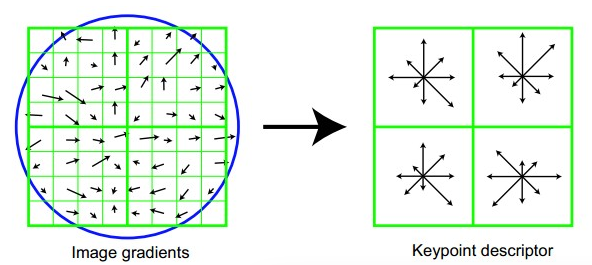
\includegraphics[width=0.5\linewidth]{sift1}
            \caption{}
            \label{fig:eight}
        \end{figure}
        
描述子采用$4×4×4=128$维向量表征,综合效果最优。
        \begin{figure}
            \centering
            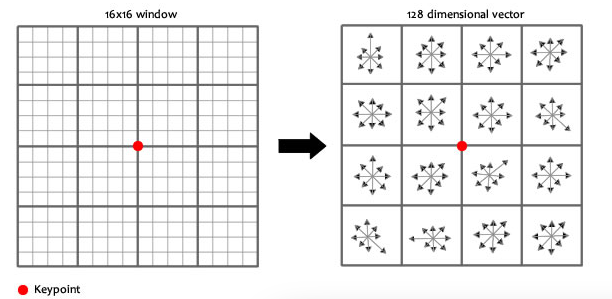
\includegraphics[width=0.5\linewidth]{sift2}
%            \caption{矩形区间和环形区间}
%            \label{fig:shape}
        \end{figure}

(4)关键点描述子产生。
\begin{enumerate}
    \item 确定计算描述子所需的图像区域,图像区域的半径通过下式计算:
        \begin{displaymath}
        radius=\frac{3\theta\_oct \times \sqrt{2} \times (d+1)}{2}
        \end{displaymath}
    \item 将坐标移至关键点主方向,如图\ref{fig:yi}。
            \begin{figure}
            \centering
            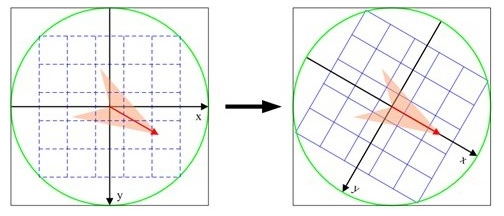
\includegraphics[width=0.5\linewidth]{yi}
            \caption{将坐标移至关键点主方向}
            \label{fig:yi}
        \end{figure}
        
        旋转后邻域内采样点的新坐标为:
        \begin{displaymath}
            \left( \begin{array}{c}
            x^{'} \\
            y^{'} \\
            \end{array} \right)
            =\left( \begin{array}{cc}
            \cos\sigma & -\sin\sigma \\
            \sin\sigma & \cos\sigma \\
            \end{array} \right)
             \left( \begin{array}{c}
            x \\
            y \\
            \end{array} \right)
        \end{displaymath}
        \item 在图像半径区域内对每个像素点求其梯度幅值和方向,然后对每个梯度幅值乘以高斯权重参数,生成方向直方图。
        \item 在窗口宽度为$2 \times 2$的区域内计算8个方向的梯度方向直方图,绘制每个梯度方向的累加值,即可形成一个种子点。然后再在下一个$2 \times 2$的区域内进行直方图统计,形成下一个种子点,共生成16个种子点。
        \item 描述子向量元素门限化及门限化后的描述子向量规范化。
        \item 根据特征点的尺度对特征描述向量进行排序,SIFT特征向量生成.
\end{enumerate}

{\color{blue}应用}:

特征点检测匹配

{\color{blue}代码}:

采用vl\_feat中的sift特征函数:
    \begin{lstlisting}[language=C++]
    [f,d] = vl_sift(img);
    \end{lstlisting}
  
\subsubsection{SURF}

SURF与SIFT算法相似,SIFT算法比较稳定,检测特征点更多,但是复杂度较高,而SURF要运算简单,效率高,运算时间短一点。

{\color{blue}算法步骤}:

(1)构建Hessian矩阵。采用的是Hessian矩阵行列式近似值图像。

(2)构造多尺度空间。

为了实现尺度不变性的特征点检测与匹配,SURF算法与SIFT算法的第一步都是构造图像多尺度空间。SURF算法则用高斯滤波与Hessian矩阵结合近似实现多尺度空间,计算复杂度相比SIFT降低多了。

(3)根据非极大值抑制初步确定特征点。

(4)主方向确定

(5)构造特征点算术描述子,SURF算法是选取一个20S(单位)的区域,分成4X4分,每一份中有5X5S,统计一份中的∑dx,∑dy,∑|dx|,∑|dy|,这样就得到$4 \times 4 \times 4 = 64$的向量描述子。SIFT是128个描述子,比SURF复杂一点。

\subsubsection{LBP}

LBP(Local Binary Pattern,局部二值模式)\footnote{\url{http://blog.csdn.net/zouxy09/article/details/7929531}}是一种用来描述图像局部纹理特征的算子;它具有旋转不变性和灰度不变性等显著的优点。它是首先由T. Ojala, M.Pietikäinen, 和 D. Harwood 在1994年提出\cite{ojala1994performance},用于纹理特征提取。而且,提取的特征是图像的局部的纹理特征。
 
 原始的LBP算子定义为在3*3的窗口内,以窗口中心像素为阈值,将相邻的8个像素的灰度值与其进行比较,若周围像素值大于中心像素值,则该像素点的位置被标记为1,否则为0。这样,3*3邻域内的8个点经比较可产生8位二进制数(通常转换为十进制数即LBP码,共256种),即得到该窗口中心像素点的LBP值,并用这个值来反映该区域的纹理信息。如下图\ref{fig:lbp}:
    \begin{figure}[!ht]
    \centering
    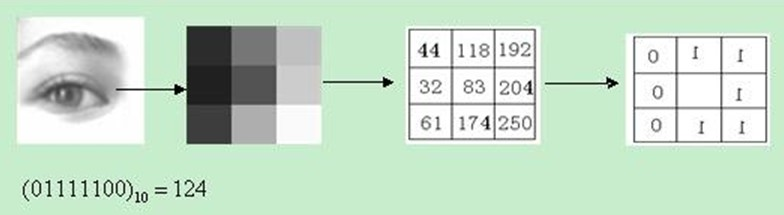
\includegraphics[width=4in]{LBP}
    \caption{LBP特征}
    \label{fig:lbp}
    \end{figure}
   
对LBP特征向量进行提取的步骤:
\begin{enumerate}
    \item 首先将检测窗口划分为16×16的小区域(cell);
    \item 对于每个cell中的一个像素,将相邻的8个像素的灰度值与其进行比较,若周围像素值大于中心像素值,则该像素点的位置被标记为1,否则为0。这样,3*3邻域内的8个点经比较可产生8位二进制数,即得到该窗口中心像素点的LBP值;
    \item 然后计算每个cell的直方图,即每个数字(假定是十进制数LBP值)出现的频率;然后对该直方图进行归一化处理。
    \item 最后将得到的每个cell的统计直方图进行连接成为一个特征向量,也就是整幅图的LBP纹理特征向量;
    \item 然后便可利用SVM或者其他机器学习算法进行分类了。
\end{enumerate}

\subsubsection{Covariance Matrix}

\subsubsection{FV(Fisher vector)}
   
Fisher vector本质上是用似然函数的梯度vector来表达一幅图像。

{\color{blue}主要思路}:用生成式模型(GMM)对样本输入进行建模,进而得到样本的一种表示(fisher vector),再将这种表示(fisher vector)输入判别式分类器(SVM)得到图像分类结果。fisher vector是fisher kernel中对样本特征的一种表示,它把一幅图片表示成一个向量。

{\color{blue}应用}:图像的分类,目标识别等领域,特别是结合着BOW model。
   
\subsubsection{GMM-HMM(Gaussian Mixture Model-Hidden Markov Model)}

{\color{blue}应用}:语音识别

\subsubsection{Gabor}

Gabor变换是D.Gabor 1946年提出的。Gabor变换属于加窗傅立叶变换,Gabor函数可以在频域不同尺度、不同方向上提取相关的特征。另外Gabor函数与人眼的生物作用相仿,所以经常用作纹理识别上,并取得了较好的效果。

Gabor滤波器是一个用于边缘检测的线性滤波器。用Gabor 函数形成的二维Gabor 滤波器具有在空间域和频率域同时取得最优局部化的特性,与人类生物视觉特性很相似,因此能够很好地描述对应于空间频率(尺度)、空间位置及方向选择性的局部结构信息。
同时,二维Gabor函数也类似于增强边缘以及峰、谷、脊轮廓等底层图像特征,这相当于增强了被认为是面部关键部件的眼睛、鼻子、嘴巴等信息,同时也增强了诸于黑痣、酒窝、伤疤等局部特征,从而使得在保留总体人脸信息的同时增强局部特性成为可能。它的小波特性说明了Gabor滤波结果是描述图像局部灰度分布的有力工具,因此,可以使用Gabor滤波来抽取图像的纹理信息。由于Gabor特征具有良好的空间局部性和方向选择性,而且对光照、姿态具有一定的鲁棒性,因此在人脸识别中获得了成功的应用。

{\color{blue}应用}:人脸识别、人脸表情识别、汉字识别

\subsubsection{DoG}



\subsubsection{DPM(Deformable Part Model)}

DPM是一个非常成功的目标检测算法,连续获得VOC(Visual Object Class)07,08,09年的检测冠军。目前已成为众多分类器、分割、人体姿态和行为分类的重要部分。2010年Pedro Felzenszwalb被VOC授予"终身成就奖"。DPM可以看做是HOG(Histogrrams of Oriented Gradients)的扩展,大体思路与HOG一致。先计算梯度方向直方图,然后用SVM(Surpport Vector Machine )训练得到物体的梯度模型(Model)。有了这样的模板就可以直接用来分类了,简单理解就是模型和目标匹配。DPM只是在模型上做了很多改进工作。

\subsubsection{GIST}

GIST是一个全局描述子,主要用于场景分类。

\subsubsection{Harris-Laplace}

\subsubsection{哈尔特征(Haar-like features)}

Haar-like特征最早是由Oren等~\cite{Pedestrian Detection Using Wavelet Templates}应用于人脸表示,Viola和Jones~\cite{Rapid
object detection using boosted cascade of simple features}在此基础上,使用3种类型4种形式的特征。

Viola等提出的Harr-like特征如图~\ref{fig: Viola_Haar-like}:

\begin{figure}[!ht]
\centering
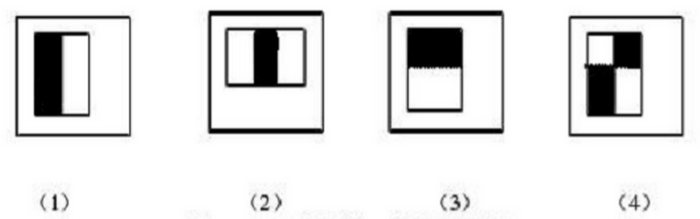
\includegraphics[width=4in]{Viola_Haar-like}
\caption{Viola提出的Haar-like特征}
\label{fig: Viola_Haar-like}
\end{figure}

将上面的任意一个矩形放到人脸区域上,然后,将白色区域的像素和减去黑色区域的像素和,得到的值我们暂且称之为人脸特征值,如果你把这个矩形放到一个非人脸区域,那么计算出的特征值应该和人脸特征值是不一样的,而且越不一样越好,所以这些方块的目的就是把人脸特征量化,以区分人脸和非人脸。

为了增加区分度,可以对多个矩形特征计算得到一个区分度更大的特征值,那么什么样的矩形特征怎么样的组合到一块可以更好的区分出人脸和非人脸呢,这就是AdaBoost算法要做的事了。

\subsubsection{ICA(Independent Component Analysis)}

独立成分分析(Independent Component Analysis, ICA)是近年来出现的一种强有力的数据分析工具(Hyvarinen A, Karhunen J, Oja E, 2001; Roberts S J, Everson R, 2001)。1994年由Comon给出了ICA的一个较为严格的数学定义,其思想最早是由Heranlt和Jutten于1986年提出来的。ICA从出现到现在虽然时间不长,然而无论从理论上还是应用上,它正受到越来越多的关注,成为国内外研究的一个热点。特别是从应用角度看,它的应用领域与应用前景都是非常广阔的,目前主要应用于盲源分离、图像处理、语言识别、通信、生物医学信号处理、脑功能成像研究、故障诊断、特征提取、金融时间序列分析和数据挖掘等。
ICA是一种用来从多变量(多维)统计数据里找到隐含的因素或成分的方法,被认为是主成分分析(Principal Component Analysis, PCA)和因子分析(Factor Analysis)的一种扩展。对于盲源分离问题,ICA是指在只知道混合信号,而不知道源信号、噪声以及混合机制的情况下,分离或近似地分离出源信号的一种分析过程。

\subsection{其它特征}

\subsubsection{local symmetry}

Reisfeld等人~\cite{}发表的论文中有关于局部对称性的描述。

Isotropic Symmetry Operator:

\begin{figure}[!ht]
 \centering
 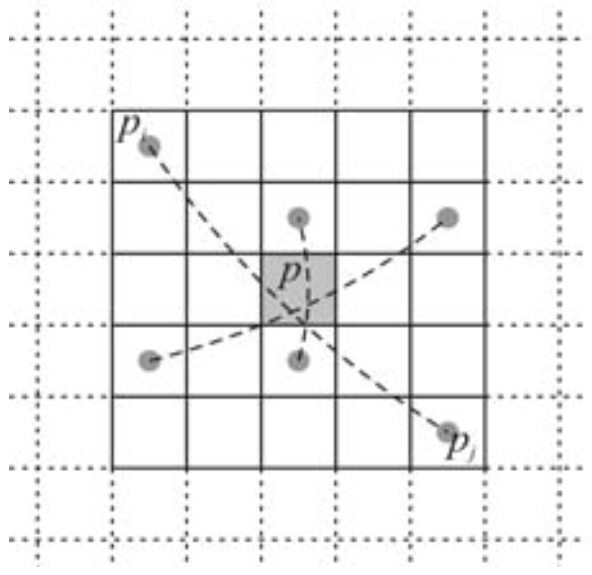
\includegraphics[width=3in]{ExamplesofPixelpairs}
\caption{用对称性算子来对像素对的梯度进行比较的三个例子}
\label{fig: ExamplesofPixelpairs}
\end{figure}

基于周围像素的灰度梯度,计算在给定点$p$处的对称性程度。如图~\ref{fig: ExamplesofPixelpairs}所示,点$p$处的对称性可以通过比较位于$p_i$和$p_j$处的像素对$i$和$j$的灰度梯度来度量,其中$p = (p_i  = p_j)/2$。每对像素对对点$p$处的局部对称性的贡献为
\begin{align}
c(i, j) = d(i, j, \sigma) \cdot p(i, j) \cdot m_i \cdot m_j
\end{align}
$m_i$是像素点$i$的梯度的模,$d(i, j, \sigma)$是当标准差为$\sigma$时,两个像素点间的距离的高斯加权函数,对称性
\begin{align}
p(i, j) = \Big(1-cos(\gamma_i+\gamma_j)\Big)\cdot \Big(1-cos(\gamma_i-\gamma_j)\Big)
\label{eq: SymmetryMeasurement}
\end{align}

其中,$\gamma_i = \theta_i-\alpha$,见图~\ref{fig: PixelpairContribution}。当点$p_i$、$p_j$关于点$p$对称时,$\gamma_i+\gamma_i=\pi$,式~(\ref{eq: SymmetryMeasurement})中的第一项取得最大值。如果只用第一项,会使得在直线边缘上的点取得较大的值,而这些点通常并不具有对称性。为了避免这个问题,又加入了第二项,表示具有相似梯度方向的像素对。最后,对所有像素对的贡献进行求和得到点$p$处的isotropic symmetry值
\begin{align}
M^{iso}(x, y) = \sum_{(i, j)\in \Gamma(p)} c(i, j)
\label{eq: IsotropicSymmetry}
\end{align}

\begin{figure}[!ht]
 \centering
 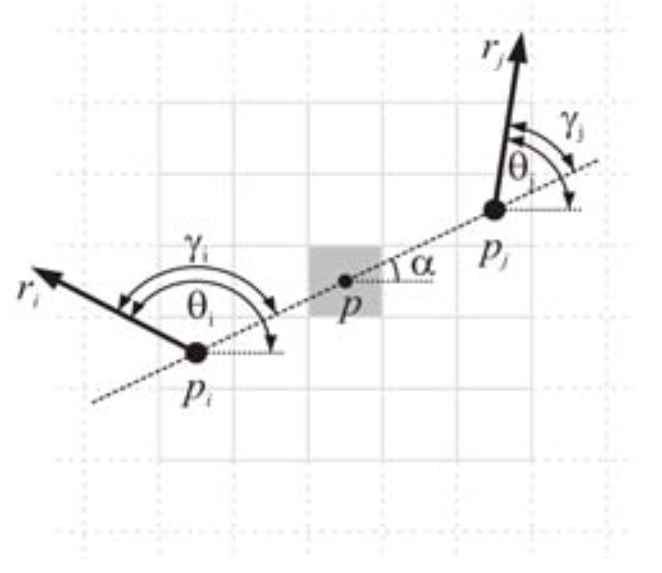
\includegraphics[width=3in]{PixelpairContribution}
\caption{每对像素对的贡献的几何表示}
\label{fig: PixelpairContribution}
\end{figure}

为了使symmetry operator对有多个对称轴的对称图案更敏感,Reisfeld等人~\cite{}又提出了radial symmetry operator,作为isotropic symmetry operator的扩展。首先,像素对的贡献的方向用$\varphi(i, j) = (\theta_i+\theta_j)/2$来计算。然后,对最大贡献为$c(i, j)$的像素对$(i, j)$,对称方向被确定为$\phi(p) = \varphi(i, j)$。这个值也用来提升有不相似方向的像素对的贡献
\begin{align}
M^{rad}= \sum_{(i, j)\in \Gamma(p)} c(i, j) \cdot sin^2(\varphi(i, j) - \phi(p))
\end{align}

\subsubsection{骨架特征}

理论:骨架又称为中轴,它的定义来自于烧草模型和最大圆盘模型。骨架不仅包含了物体的几何特征,也描述了物体的拓扑结构。经典的骨架化算法有中轴变换、细化算法、Voronoi图算法等。在骨架的基础上可以通过奇点图、骨架树等对物体的结构特征进行描述。

骨架树:将骨架映射到一个树状结构(如图\ref{fig:tree})。仅有一个邻接点的骨架点成为端点,有两个以上邻接点的骨架点称为分支点,骨架上除了分支点和端点外的点称为连接点。
        \begin{figure}
            \centering
            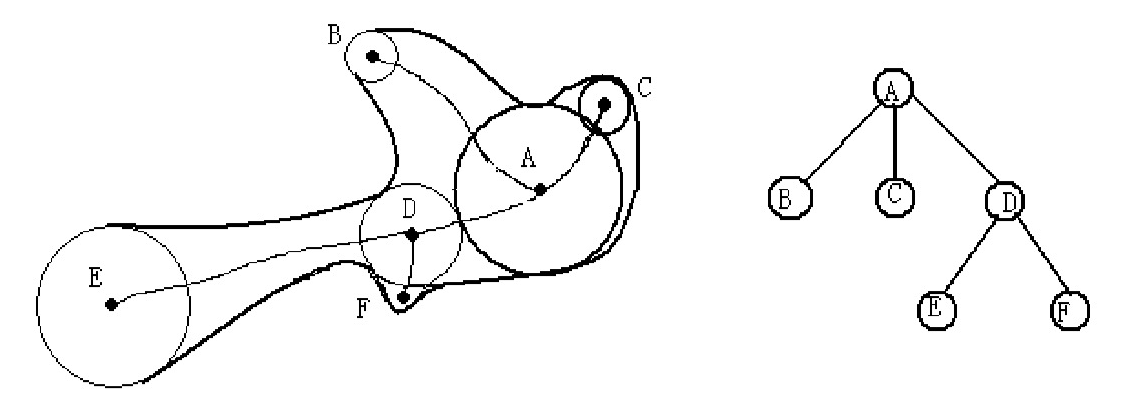
\includegraphics[width=0.5\linewidth]{tree}
            \caption{骨架树}
            \label{fig:tree}
        \end{figure}
        根据骨架树深度优先搜索产生的节点序列中的所有节点用其孩子数替换,替换后得到的新序列即为树描述符。例如,图\ref{fig:tree}的树描述符为(3,2,0,0,0,0)。

骨架化代码:\url{http://cs.smith.edu/~nhowe/research/code/}。

\subsubsection{灰度特征}

1)灰度直方图
灰度直方图是灰度级函数,它表示图像中每种灰度级的像素的个数,反映图像中每种灰度出现的频率。灰度直方图的横坐标是灰度级,纵坐标是该灰度级出现的频率。

    \begin{lstlisting}[language=C++]
    imhist(I,n);
    \end{lstlisting}
    
2)灰度共生矩阵(GLCM)

灰度共生矩阵是对图像上保持某距离的两像素分别具有某种灰度的情况进行统计得到的。它不仅反映亮度的分布特性,也
反映具有同样亮度或接近亮度的像素之间的位置分布特性。对灰度共生矩阵的理解,需要明确几个概念:方向、偏移量和灰度共生矩阵的阶数。
\begin{description}
    \item[方向] 一般计算过程会分别选在几个不同的方向来进行,通常为0,45,90,135。
    \item[偏移量] 
    \item[灰度共生矩阵阶数] 灰度共生矩阵的阶数和灰度图像灰度值的阶数是一致的,即当灰度图像灰度值的阶数是$N$时,灰度共生矩阵为$N \times N$。
\end{description}

 取图像($N \times N$)中任意一点(x,y)及偏离它的另一点(x+a,y+b),设该点对的灰度值为(g1,g2)。令点(x,y)在整个画面上移动,则会得到各种(g1,g2)值,设灰度值的级数为256,则(g1,g2)的组合共有256*256种(共生矩阵的大小)。对于整个画面,统计出每一种(g1,g2)值出现的次数,然后排列成一个方阵,在用(g1,g2)出现的总次数将它们归一化为出现的概率$P(g1,g2)$,这样的方阵称为灰度共生矩阵。
 
 为了能更直观的以共生矩阵描述纹理情况,从共生矩阵导出一下反映矩阵情况的参数,典型的有一下几种:
 \begin{description}
     \item[能量] 为灰度共生矩阵元素值的平方和,反映了图像灰度分布均匀程度和纹理粗细度。ASM值大表明一种较均一和规则变化的纹理模式。
         \begin{displaymath}
             ASM=\sum_{i=0}^{k}\sum_{j=0}^{k}G(i,j)^{2}
         \end{displaymath}
     \item[对比度] 反映了某个像素值及其领域像素值的亮度的对比情况。如果偏离对角线的元素有较大值,即图像亮度值变化很快,则CON会有较大取值。
         \begin{displaymath}
             CON=\sum_{i}\sum_{j}(i-j)^{2}G(i,j)
         \end{displaymath}
     \item[熵] 表示图像的信息量,当共生矩阵中所有元素有最大的随机性、空间共生矩阵中所有值几乎相等时,共生矩阵中元素分散分布时,熵较大。它表示了图像中纹理的非均匀程度或复杂程度。 
         \begin{displaymath}
             ENT=\sum_{i}\sum_{j}G(i,j)\log G(i,j)
         \end{displaymath}
     \item[自相关] 反应了图像纹理的一致性。如果图像中有水平方向纹理,则水平方向矩阵的COR大于其余矩阵的COR值。
         \begin{displaymath}
             COR=\frac{\sum_{i}\sum{j}[(ij)G(i,j)]-u_{i}u_{j}}{s_{i}s_{j}}
         \end{displaymath}
 \end{description}
 
    \begin{lstlisting}[language=C++]
    [glcm,SI] = graycomatrix(Img);
    \end{lstlisting}

\subsubsection{凸包}


\subsubsection{SC}
    
    SC\cite{belongie2002shape}(Shape context,形状上下文)是基于物体轮廓样本点进行描述的。
    
    {\color{blue}主要思想}:用直方图描述轮廓上点间的位置关系。
    
    {\color{blue}算法步骤}:
    \begin{enumerate}
        \item 边缘提取(如图\ref{fig:edge})。
           \begin{figure}
            \centering
              \begin{minipage}[t]{0.2\linewidth}
              \centering
              
\includegraphics[width=0.6\linewidth]{a1} 
              \caption{原始图像}
              \label{fig:org}
              \end{minipage}
              \begin{minipage}[t]{0.2\linewidth}
              \centering
              \includegraphics[width=0.6\linewidth]{a-edge}
              \caption{边缘提取}
              \label{fig:edge}
              \end{minipage}
              \begin{minipage}[t]{0.2\linewidth}
              \centering
              \includegraphics[width=0.6\linewidth]{a-point}
              \caption{采样点}
              \label{fig:point}
              \end{minipage}
            \end{figure}    
        \item 从边缘上均匀采样n个点,得到一个物体形状的点集合(如图\ref{fig:point})。
        \item 通过对数极坐标空间(如图\ref{fig:log})计算每个采样点与形状其他点之间的位置关系,采用直方图表示(如图\ref{fig:his})。n个采样点中,每个点都有一个直方图对其位置进行描述。
           \begin{figure}
            \centering
              \begin{minipage}[t]{0.4\linewidth}
              \centering
              \includegraphics[width=0.6\linewidth]{a-log} 
              \caption{对数极坐标空间}
              \label{fig:log}
              \end{minipage}
              \begin{minipage}[t]{0.47\linewidth}
              \centering
              \includegraphics[width=0.6\linewidth]{his}
              \caption{直方图}
              \label{fig:his}
              \end{minipage}
            \end{figure}  
    \end{enumerate}
    但由于形状上下文不能很好地解决物体类内部之间的变形,因此采用基于内部距离的形状上下文\cite{ling2007shape},内距离形状上下文中采用内距离代替欧式距离。
    
内距离形状上下文代码:\url{http://www.dabi.temple.edu/~hbling/code_data.htm}。



田奇

binary feature descriptors

\subsubsection{Binary SIFT (BSIFT) – Zhou, TIP 2014}

\subsubsection{COGE - PCM 2013 Best Paper, Mao , 2013}

\subsubsection{Ultra-Short Binary Descriptor (USB) – Zhang S., TIP , 2014}

\subsubsection{Topology-Preserving Hashing – Zhang L., MM 2012}


\section{学习算法}


\subsection{随机森林}

“视觉机器学习20讲”中提供了随机森林的源代码,是c与matlab的混合编程,但是只有在windows下编译好了的文件,在mac下无法跑。

DRFI方法中用到随机森林\footnote{\url{https://code.google.com/p/randomforest-matlab/}}学习方法,下载下来解压后是在randomforest-matlab文件夹中,其中又包含两个文件夹,一个是RF\_Class\_C,用来做分类的,另一个是RF\_Reg\_C,用来做回归的。

RF\_Class\_C文件夹中需要对.cpp文件进行编译,生成mexmaci64文件,这一步可以通过在终端输入make mex命令实现。但是可能由于我电脑中的fortran版本不行,编译总是出错,目前还没有解决,后来在网页上\footnote{\url{https://code.google.com/p/randomforest-matlab/issues/detail?id=54}}搜到了已编译好的mexmaci64文件,可以直接拿过来用。

tutorial\_ClassRF.m文件列举了10个例子,展示了用不同的参数跑随机森林学习算法的不同结果。

\subsection{SVM}

\subsection{Bayes}

\subsection{K-means}

\subsection{Decision tree}

\subsection{EM(Expectation Maximization Algorithm)}
最大期望(EM)算法是在概率(probabilistic)模型中寻找参数最大似然估计或者最大后验估计的算法,其中概率模型依赖于无法观测的隐藏变量(Latent Variable)。最大期望经常用在机器学习和计算机视觉的数据聚类(Data Clustering)领域。

\subsection{KNN}

\subsection{Ensemble learning}

\subsubsection{AdaBoost}

\subsubsection{Bagging}

\subsubsection{Gasen}






%
% references
\bibliographystyle{plain}

\bibliography{zooplankton} %参考文献


\end{document}